% !TEX root = 99_main.tex

%This section is now called 'Case Study'

This section details some of the outcomes of the aforementioned design environment in relation to the case study at the HiLo building. In particular we will evaluate the optimal PV panel layout, the structure, details of the module design, and fabrication.

\subsection{Optimum PV Panel Layout}
The design of the PV panel layout is an example where all four stakeholders had inputs to the design. From an energetic perspective, a dense layout would have a larger overall PV surface area for electricity generation. However if the panels are too close together, there would be high module self shading which would lower the overall performance of the panels, as seen in Figure \ref{fig:spacing} \cite{hofer2016parametric}. Furthermore, there would be less natural lighting in the room,resulting in an increase of the building's overall  energy consumption. From an architectural perspective, a sparse PV layout is preferred as it increases the transparency of the facade from the inside. This also lowers the overall cost, as less PV panels are required. Structurally, however, a sparse PV layout results in longer pipe elements between the junctions which lowers the overall strength, due to increased buckling length. Ultimately, a PV panel spacing of 510mm with a module size of 420mm was chosen as a trade-off between the above mentioned requirements. 

\begin{figure}
\begin{center}
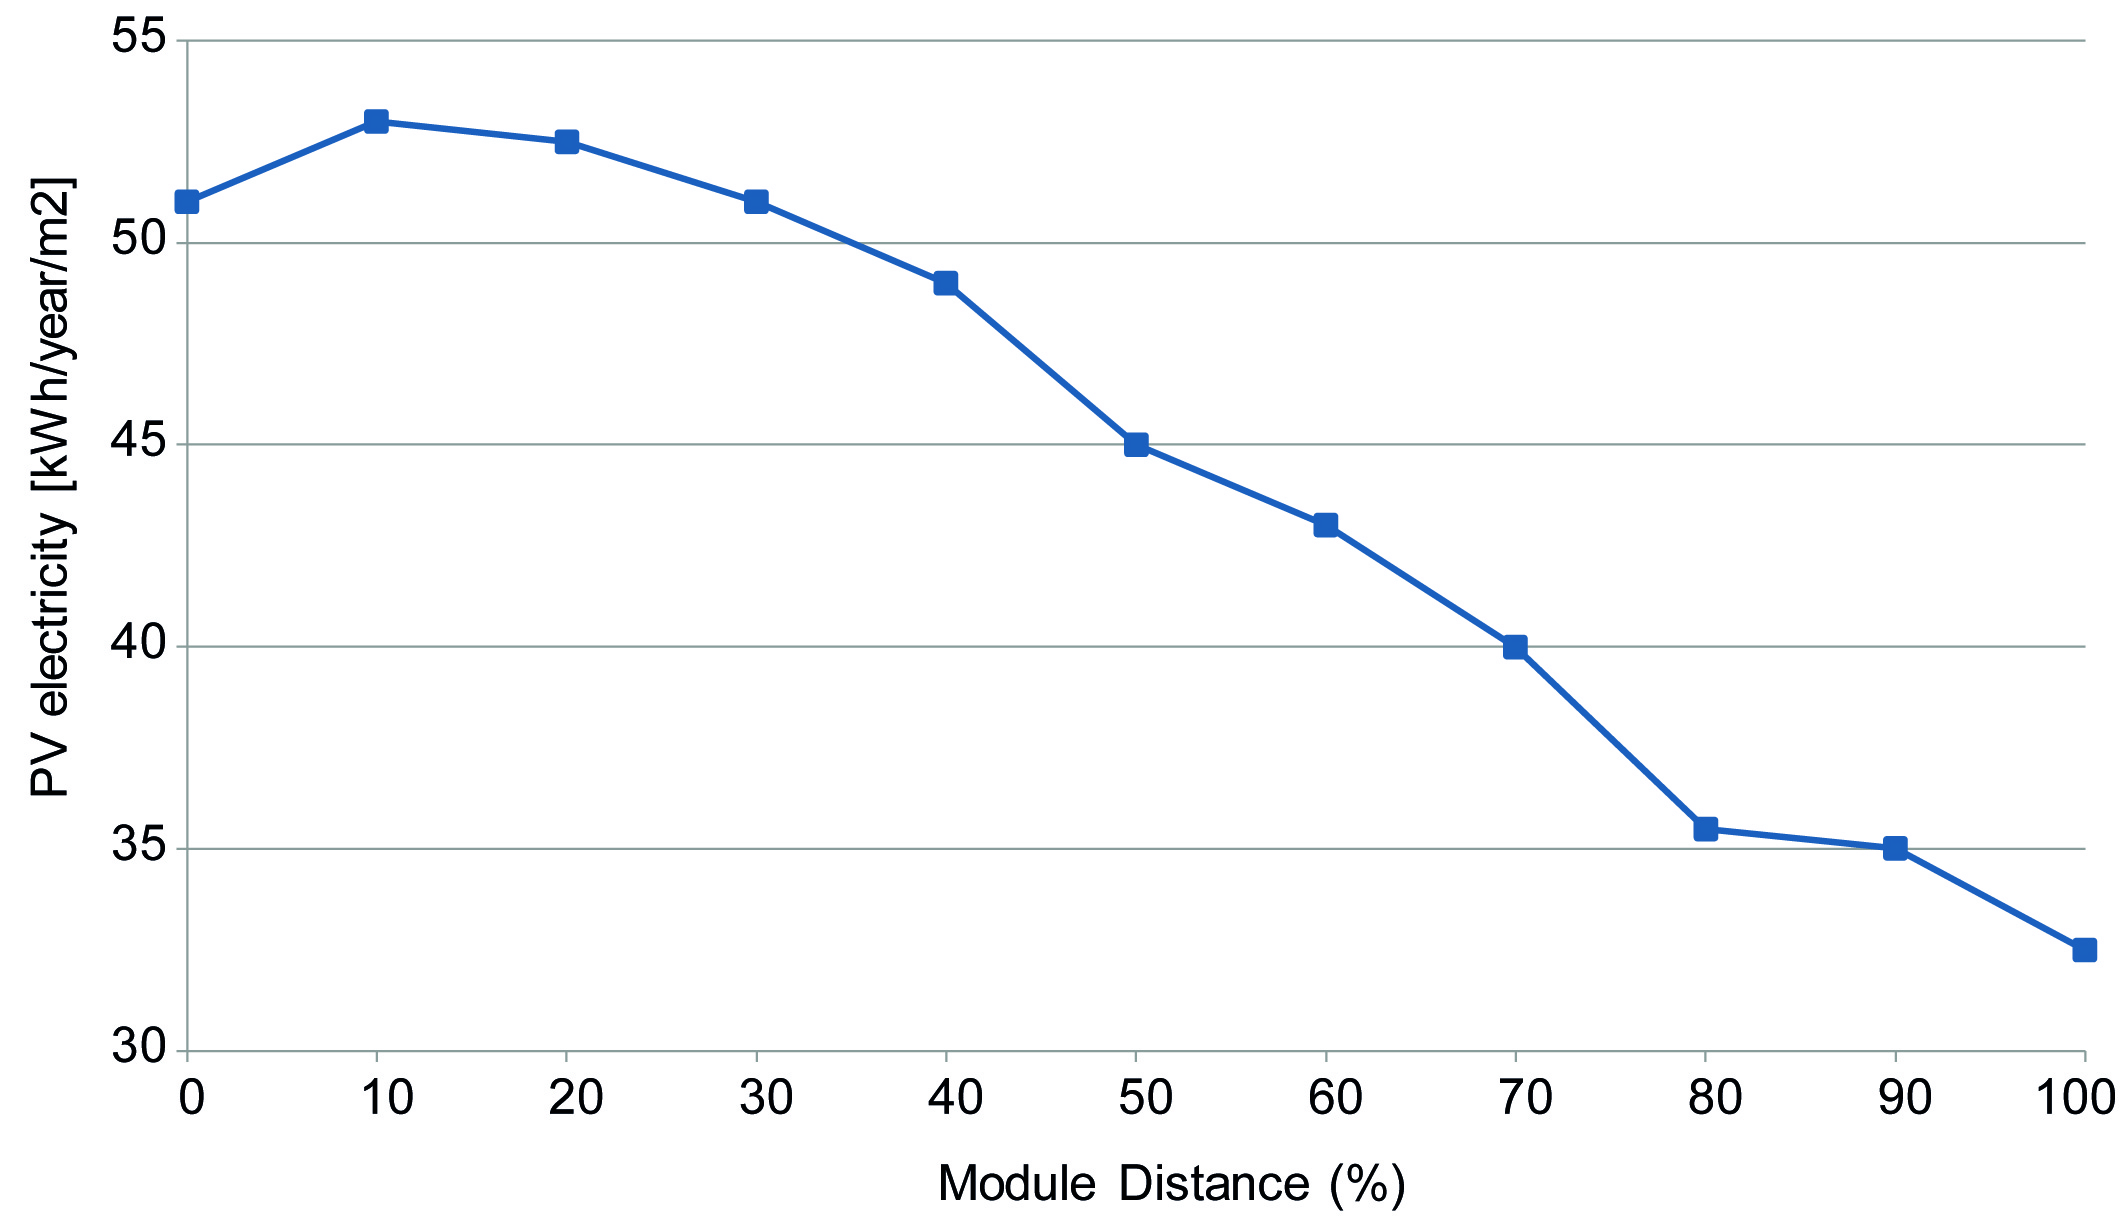
\includegraphics[width=0.8\columnwidth, trim= 0cm 0cm 0cm 0cm,clip]{ASF_PV_Distance-07.jpg}
\caption{Effect of annual PV production with respect to module spacing per square meter of facade area \cite{hofer2016parametric}}
\label{fig:spacing}
\end{center}
\end{figure}

\subsection{Optimum Supporting Frame Dimension}
\label{ch:structure}


With a frame size of 2.5 x 4.02 m, a PV panel spacing of 510 mm and a structural depth of the vault of 150 mm, the shape of the rod-net vault, the profiles  of the pipes, and the size of the supporting frame was calculated. With a wind load of 0.92KN /m2, and a safety factor of 1.8, the finite element analysis concluded that the stainless steel pipe and the rectangular steel frame have a minimum dimensions of 16x2mm and 180x120x6mm respectively. 

The relatively large frame is the result of a snap-through buckling failure criterion and relatively weak support conditions at the corners. As the vault is loaded, the large lateral forces on the frame result in deflections, which in turn reduce the depth of the vaulted structure. The reduced depth of the vault further increases the lateral loading, thus leading to a global snap-through buckling failure. The frame must therefore be large enough to withstand the maximum load criterion with minimal deflection. This solution is characteristic to the conditions present on the HiLo building, where the ASF will be mounted with an offset of 80 cm from the building's support structure. In principle, the edge point of the pipe structure could be mounted directly to the support structure of the building, thus reducing the need for a frame. Figure \ref{fig:frameSize} depicts how the utilisation of the pipe elements decreases with increasing frame strength, up to the point where all edge points are supported individually. 

The 150 mm depth of the vaulted structure is sufficient to handle the wind loads with relatively thin pipes and minimal variation in the panel orientation. Ultimately, the choice of the structural depth is a trade-off between stability,  self-shading, and aesthetics. A deeper structure offers more load bearing capacity requiring thinner pipes, however the self-shading of the panels increase. On the other hand, a shallow structure is less resilient to wind loads, leading to thicker pipes. The effect of the depth on the structural stability is depicted in Figure \ref{fig:StructuralDepth}. The figure shows how the maximum utilisation of the pipes decreases with increasing structural depth, with a very steep decrease in the range of 12-15 cm. 

The construction details contribute significantly to the overall stability of the structure and to the match between the real behaviour and the FEA simulation. For this reason, we designed the pipe and frame connections to provide a completely stiff connection under the assumed wind loads. To form the vaulted shape, each pipe element is bent close to its edges and kept straight in between those points to improve their stability to localised buckling.


\begin{figure}
    \centering
    \begin{subfigure}[b]{0.8\columnwidth}
        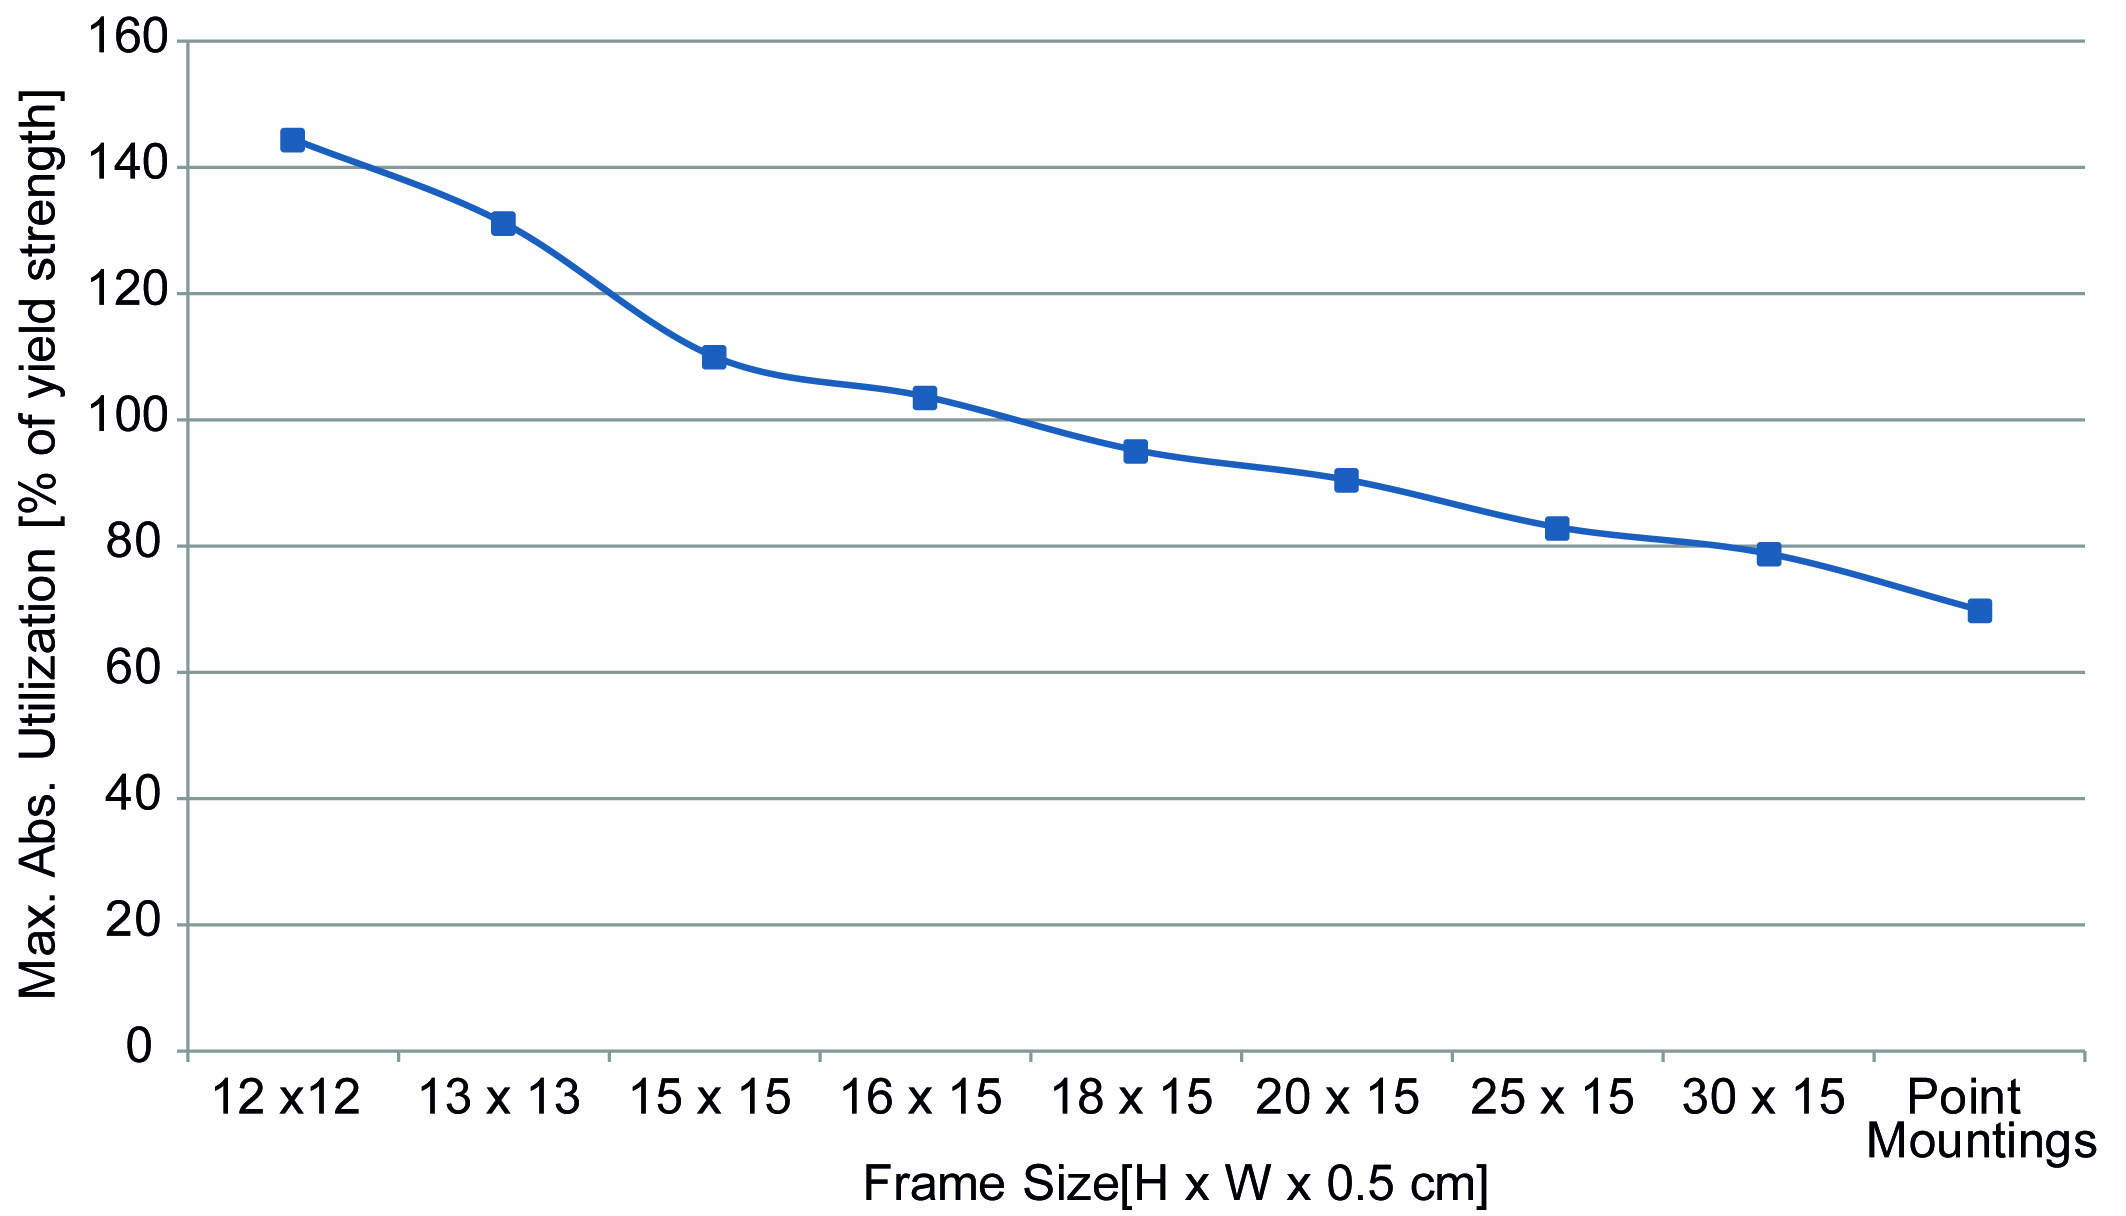
\includegraphics[width=\textwidth]{ASF_Utilisation_FrameSize-09.jpg}
        \caption{} 
        \label{fig:frameSize}
    \end{subfigure} 
    \vspace{10mm}

    \begin{subfigure}[b]{0.8\columnwidth}
        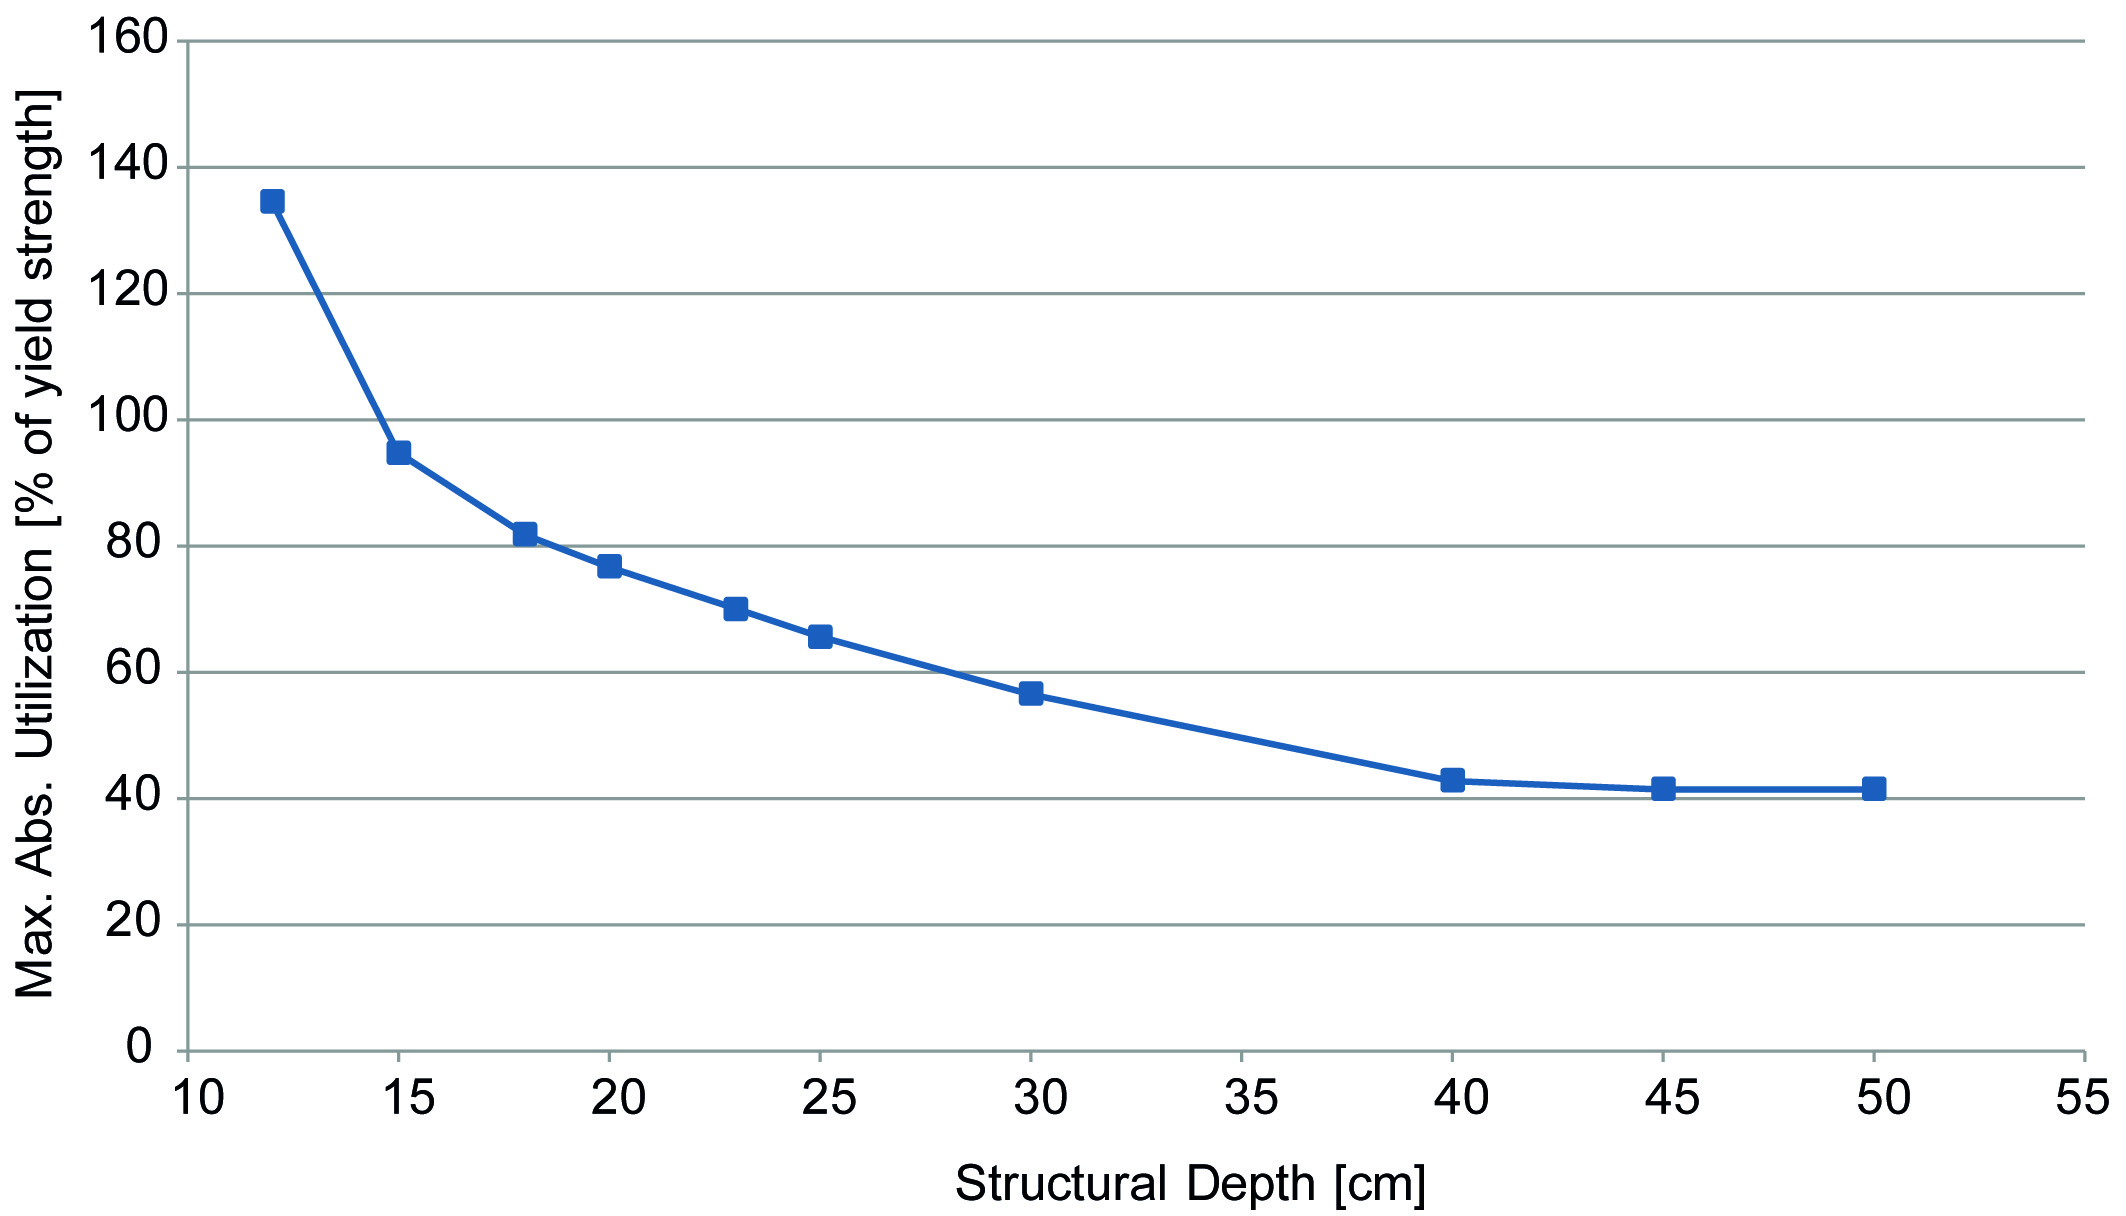
\includegraphics[width=\textwidth]{ASF_Utilisation_Depth-08.jpg}
        \caption{}
        \label{fig:StructuralDepth}
    \end{subfigure}
    \hfill

    \caption{Utilisation factor, represented as a percentage of the maximum yield strength. Failure occurs with utilisation factors greater than 100\%. The utilisation factor decreases with increasing frame size cross section, and with greater vaulted depth.}
    \label{fig:utilisation}
\end{figure}

\subsection{Structural Validation}

Due to the complexity of the joints and double curved form, it was important to validate the structural analysis. A scaled down, 2.2m x 1.5m, prototype designed through the PDE was constructed for testing purposes. Weights were added to each of the seven junction nodes in 5kg increments until the structure collapsed as seen in Figure \ref{fig:validation}. Each junction node was also fitted with a deflection gauge.

The results of this analysis are summarised in Table \ref{tab: validation}. The simulated model underestimates the overall strength by 12\% which is sufficient to validate our model. The deflection results, however, have a larger diversion. This diversion can be attributed to a weak construction joint at one of the edge nodes. The average deflection of the structure is 10.5mm which is close to the simulated model. Besides confirming the accuracy of the simulation, this test also confirmed the predicted snap-though buckling failure. Additionally, as seen in Figure \ref{fig:failure2}, the junction nodes, and frame connections were capable of resisting local torsion and maintained their position. The failure was localised at the pipes as predicted in Section \ref{ch:structure}. 

\begin{figure}
    \centering
    \begin{subfigure}[b]{0.47\textwidth}
        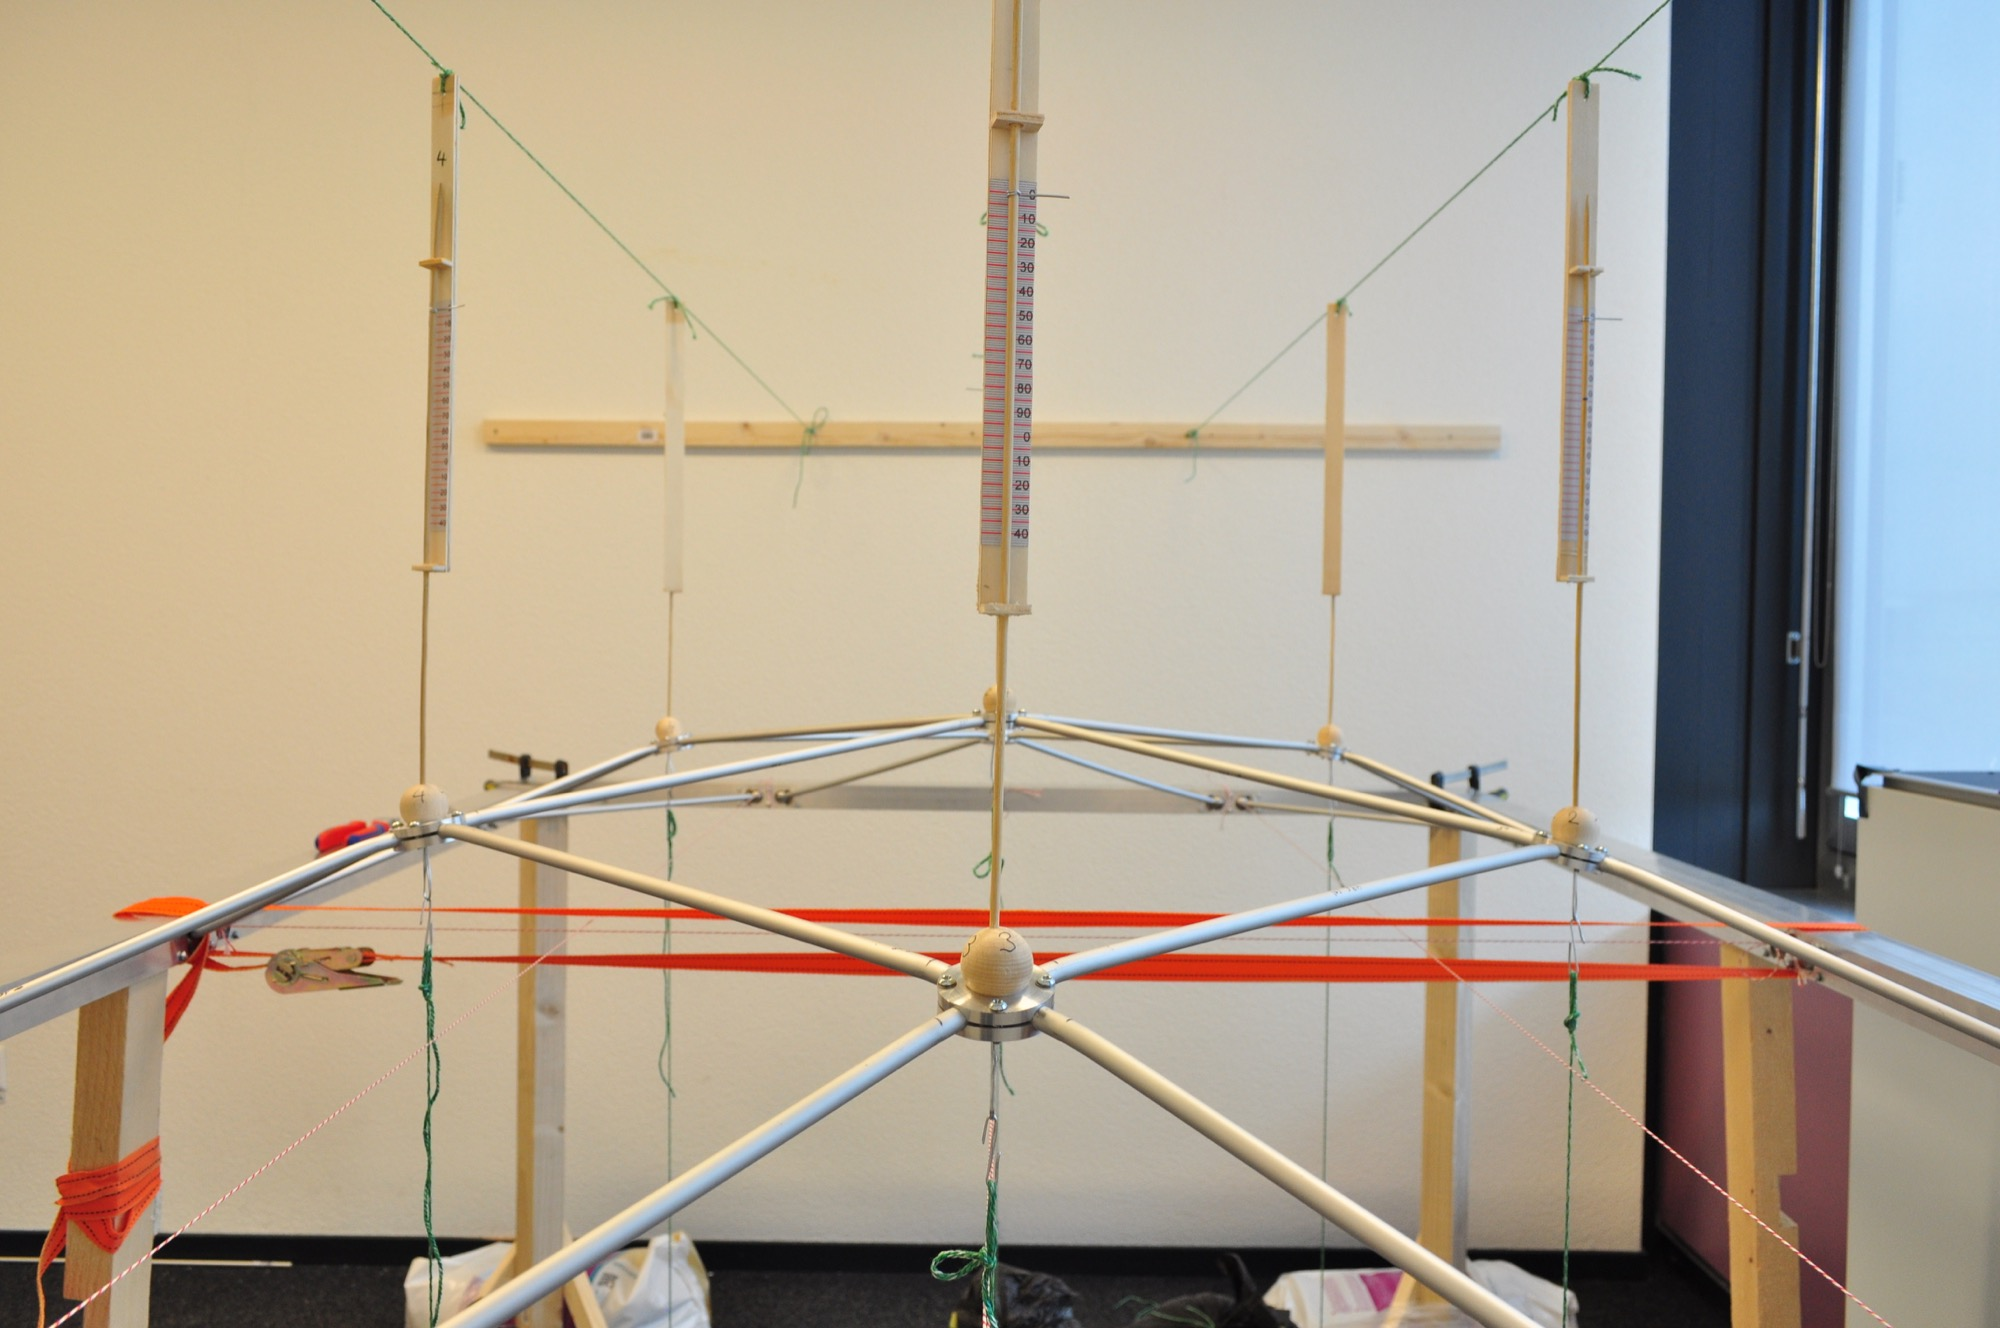
\includegraphics[width=\textwidth]{validation2.JPG}
        \caption{} 
        \label{fig:validation1}
    \end{subfigure} 
    \begin{subfigure}[b]{0.47\textwidth}
        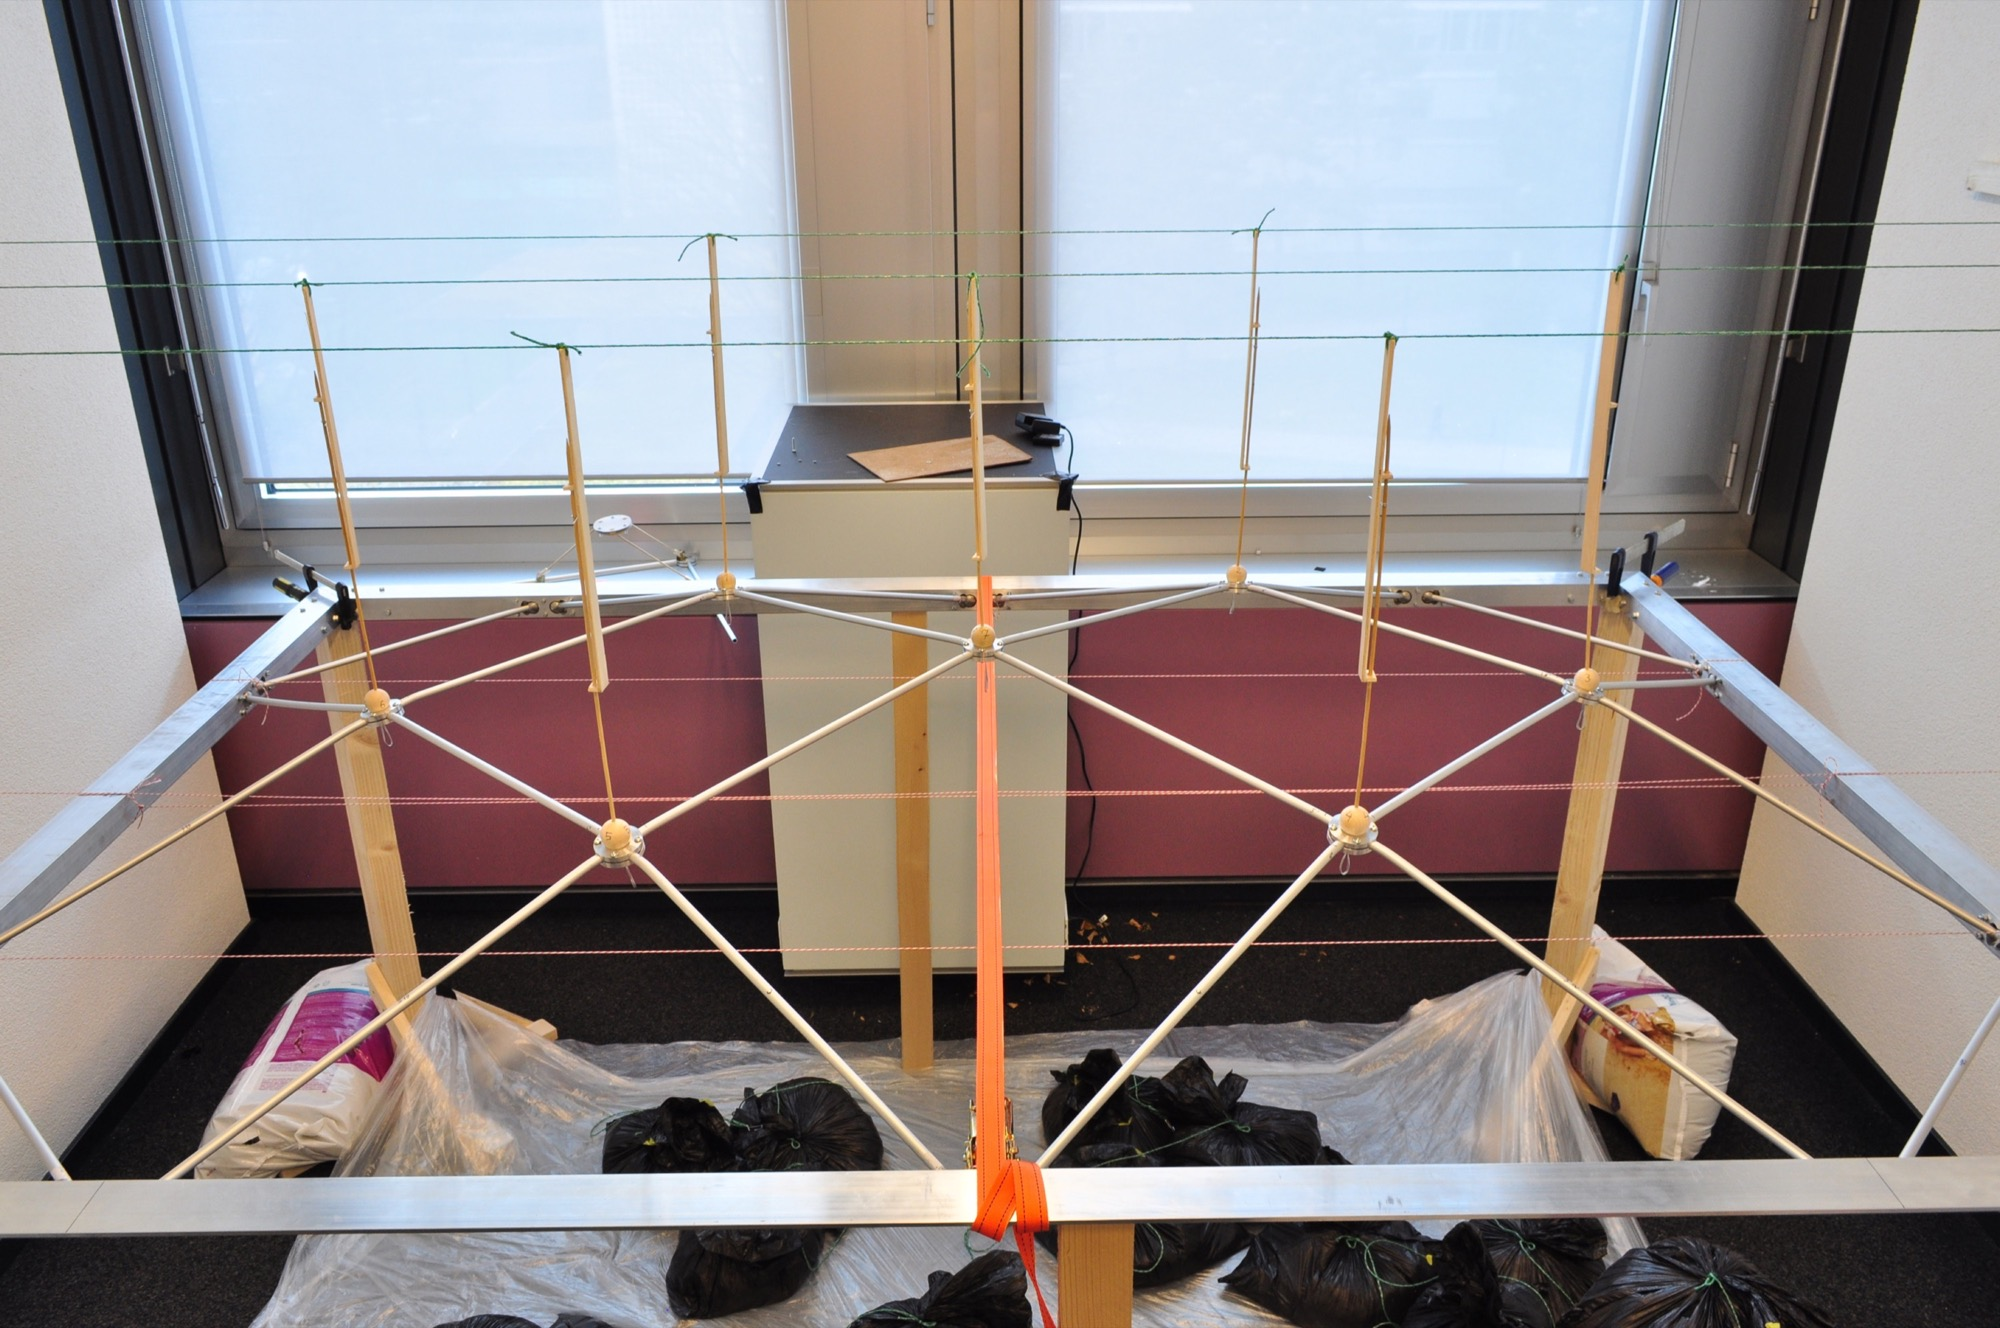
\includegraphics[width=\textwidth]{validation1.JPG}
        \caption{}
        \label{fig:validation2}
    \end{subfigure}
    \hfill
        \begin{subfigure}[b]{0.47\textwidth}
        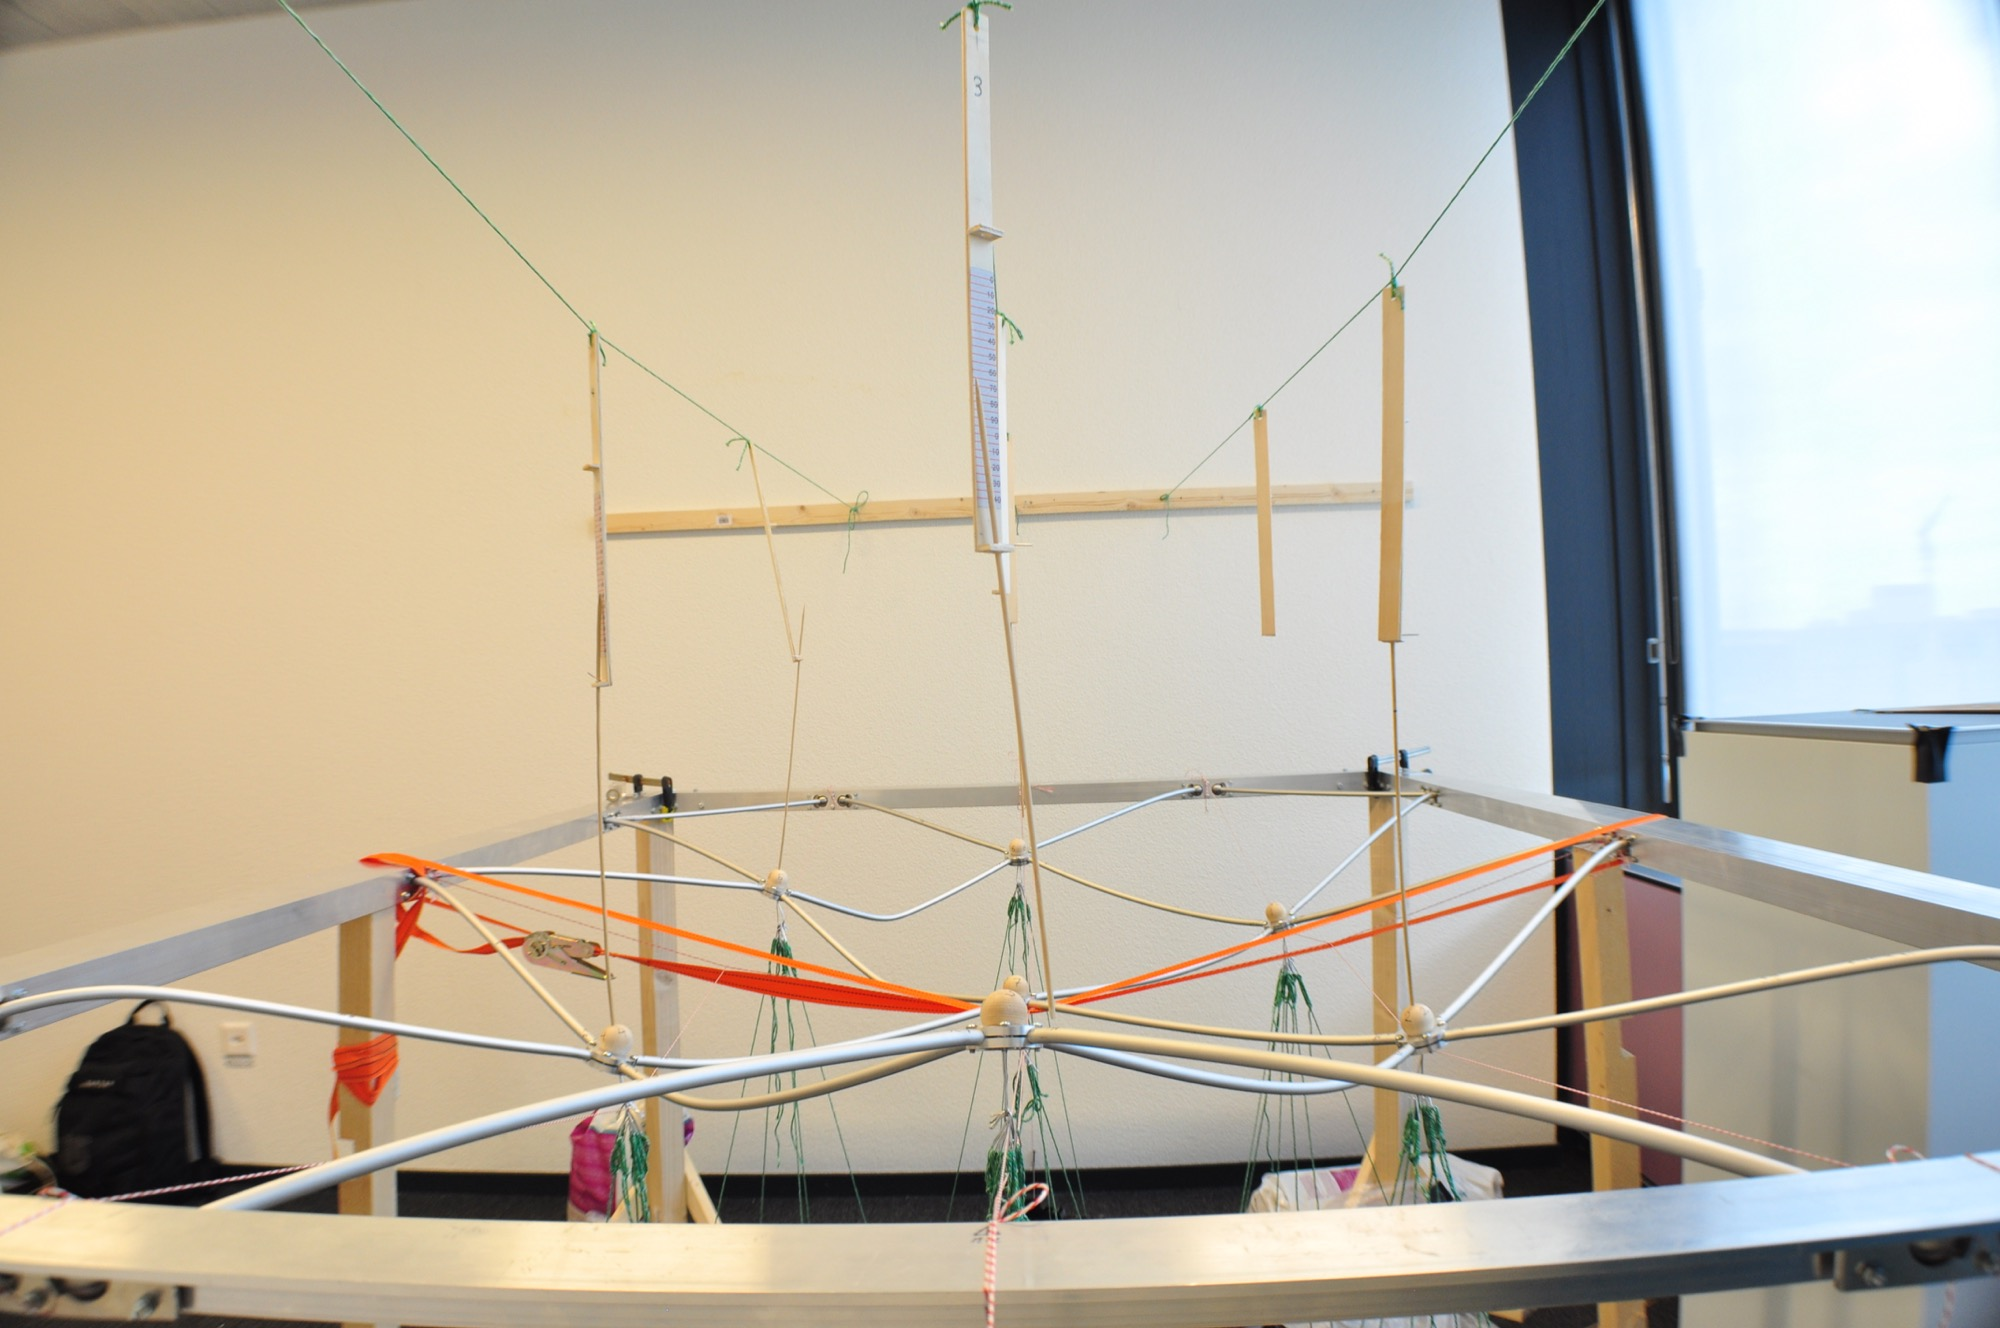
\includegraphics[width=\textwidth]{failure1.JPG}
        \caption{} 
        \label{fig:failure1}
    \end{subfigure} 
    \begin{subfigure}[b]{0.47\textwidth}
        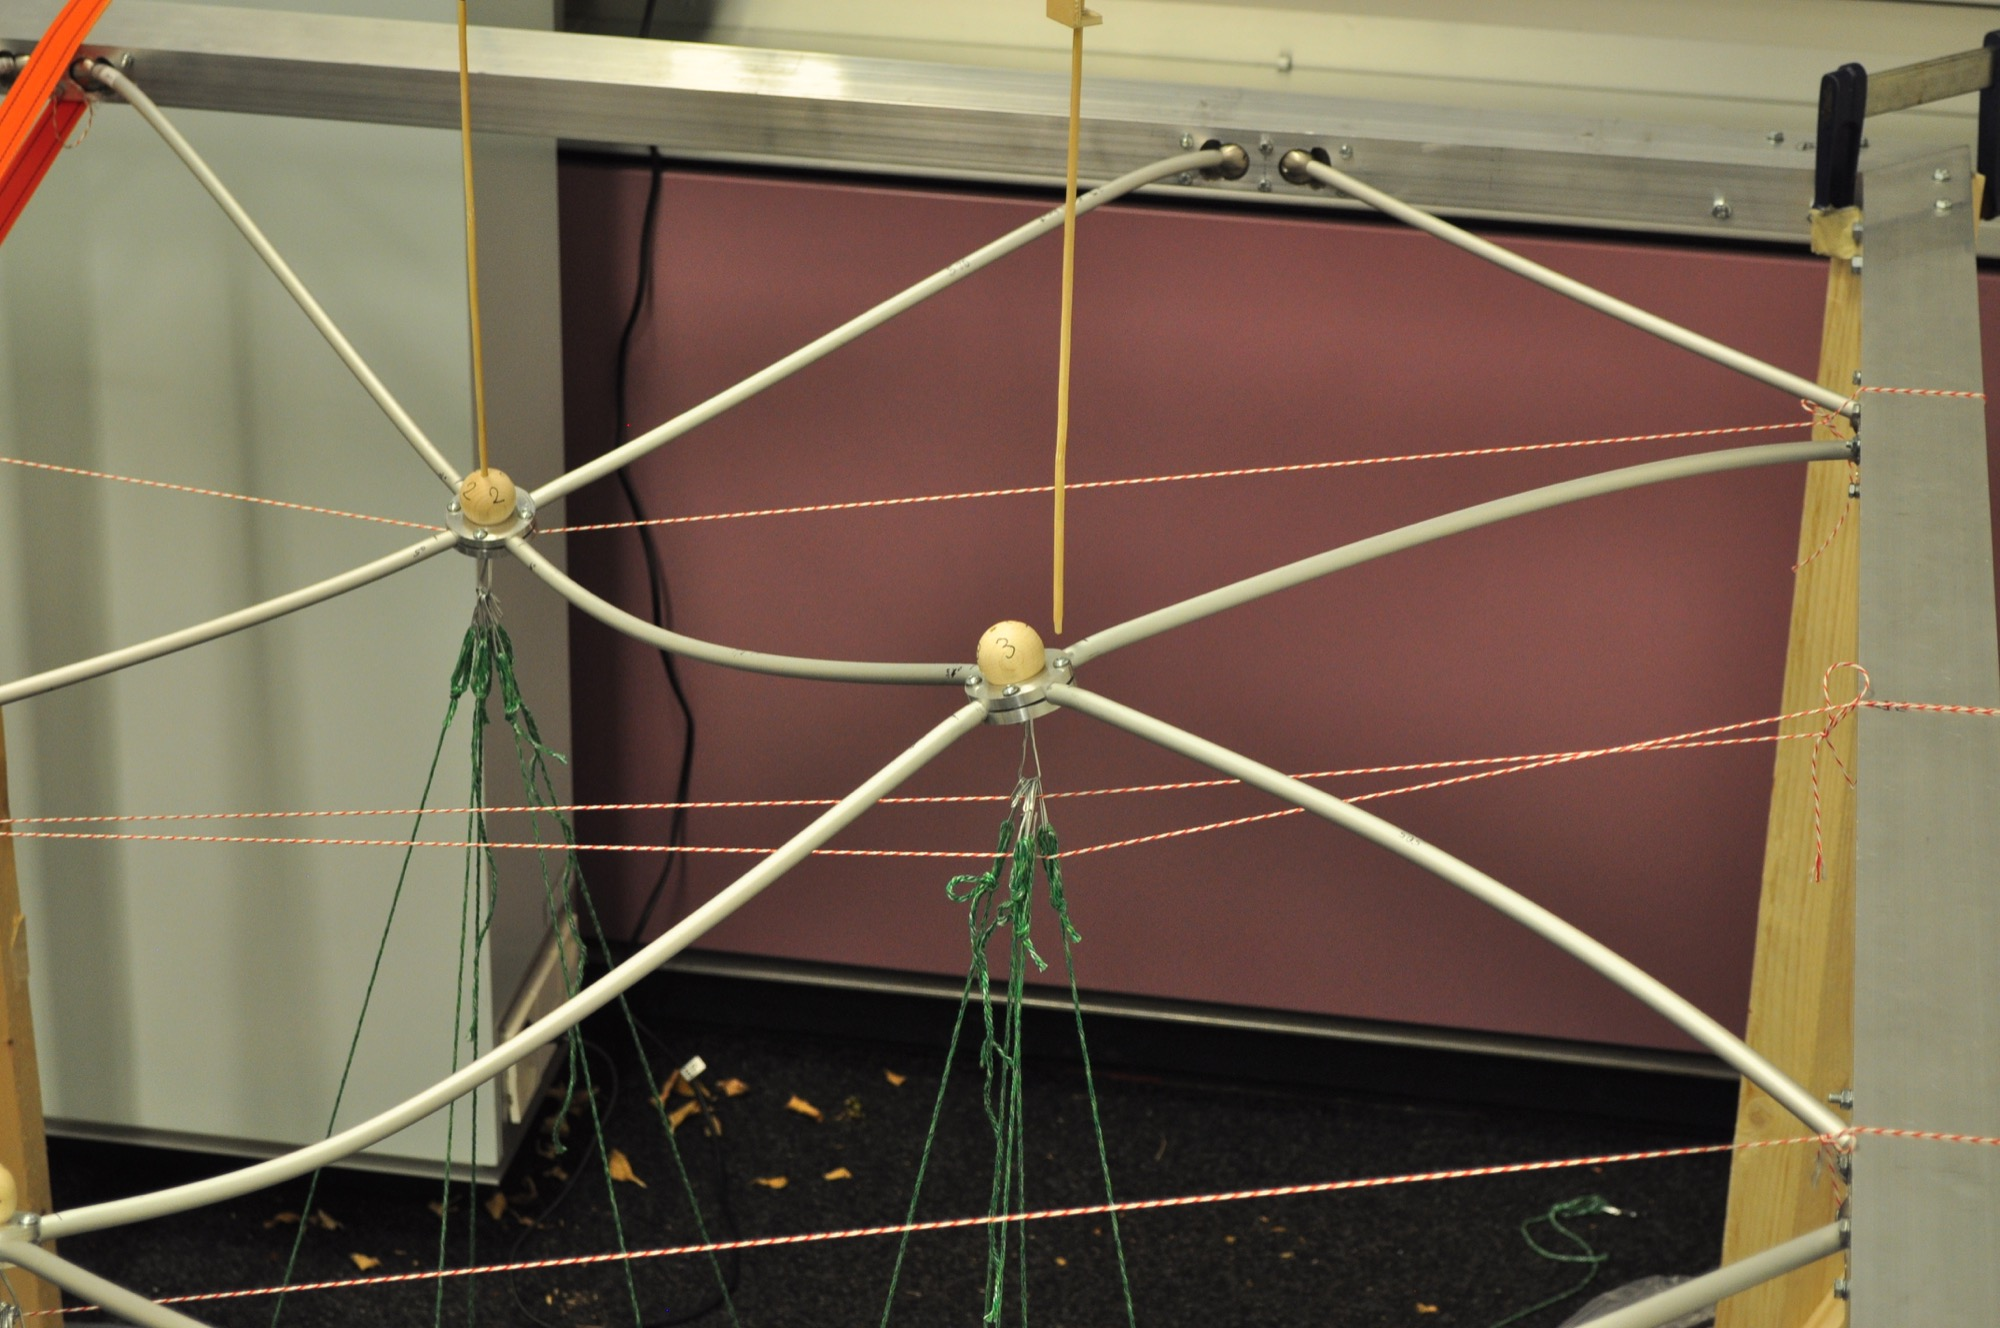
\includegraphics[width=\textwidth]{failure2.JPG}
        \caption{}
        \label{fig:failure2}
    \end{subfigure}

    \caption{Prototype constructed for model validation. a,b details the experimental set up. c,d detail the snap-through buckling of the structure}
    \label{fig:validation}
\end{figure}

\begin{table}
\begin{tabular}{llll}
                                 & Physical Model & Simulated Model & Deviation \\
\hline
Max Point Loading & 250N           & 220N   & -12\%         \\
Max Deflection & 14.5mm         & 10.3mm  & -29\%        \\
\hline
\end{tabular}
\caption{Comparison of the physical and simulated model for the scaled down prototype}
\label{tab: validation}
\end{table}

\subsection{Module Design}

The kinetic PV module was then parametrically designed to fit within the requirements of the optimised layout and structure. The PV panels must be able to fully open, and fully close without making contact with the rod-net structure or other PV modules as shown in Figure \ref{fig:constraints}. The PV panel is actuated using a soft pneumatic actuator \cite{Svetozarevic2017a}. The actuator is made from neoprene rubber and contains three air chambers. By pumping one or more of these chambers with compressed air, the actuator will deform, thus moving the panel with a 90$^{\circ}$ range in two degrees of freedom. The cantilevered bracket connects this actuator to the rod-net structure and holds it at a distance that prevents collision with other PV panels or the structure. A decentralised control box, located behind the junction element, contains three pneumatic valves and an electronic board addresses the valves over a common data bus. This controls the flow of air to the chambers inside the actuator. An exploded view of the module is shown in Figure \ref{fig:exploded}.


\begin{figure}
\begin{center}
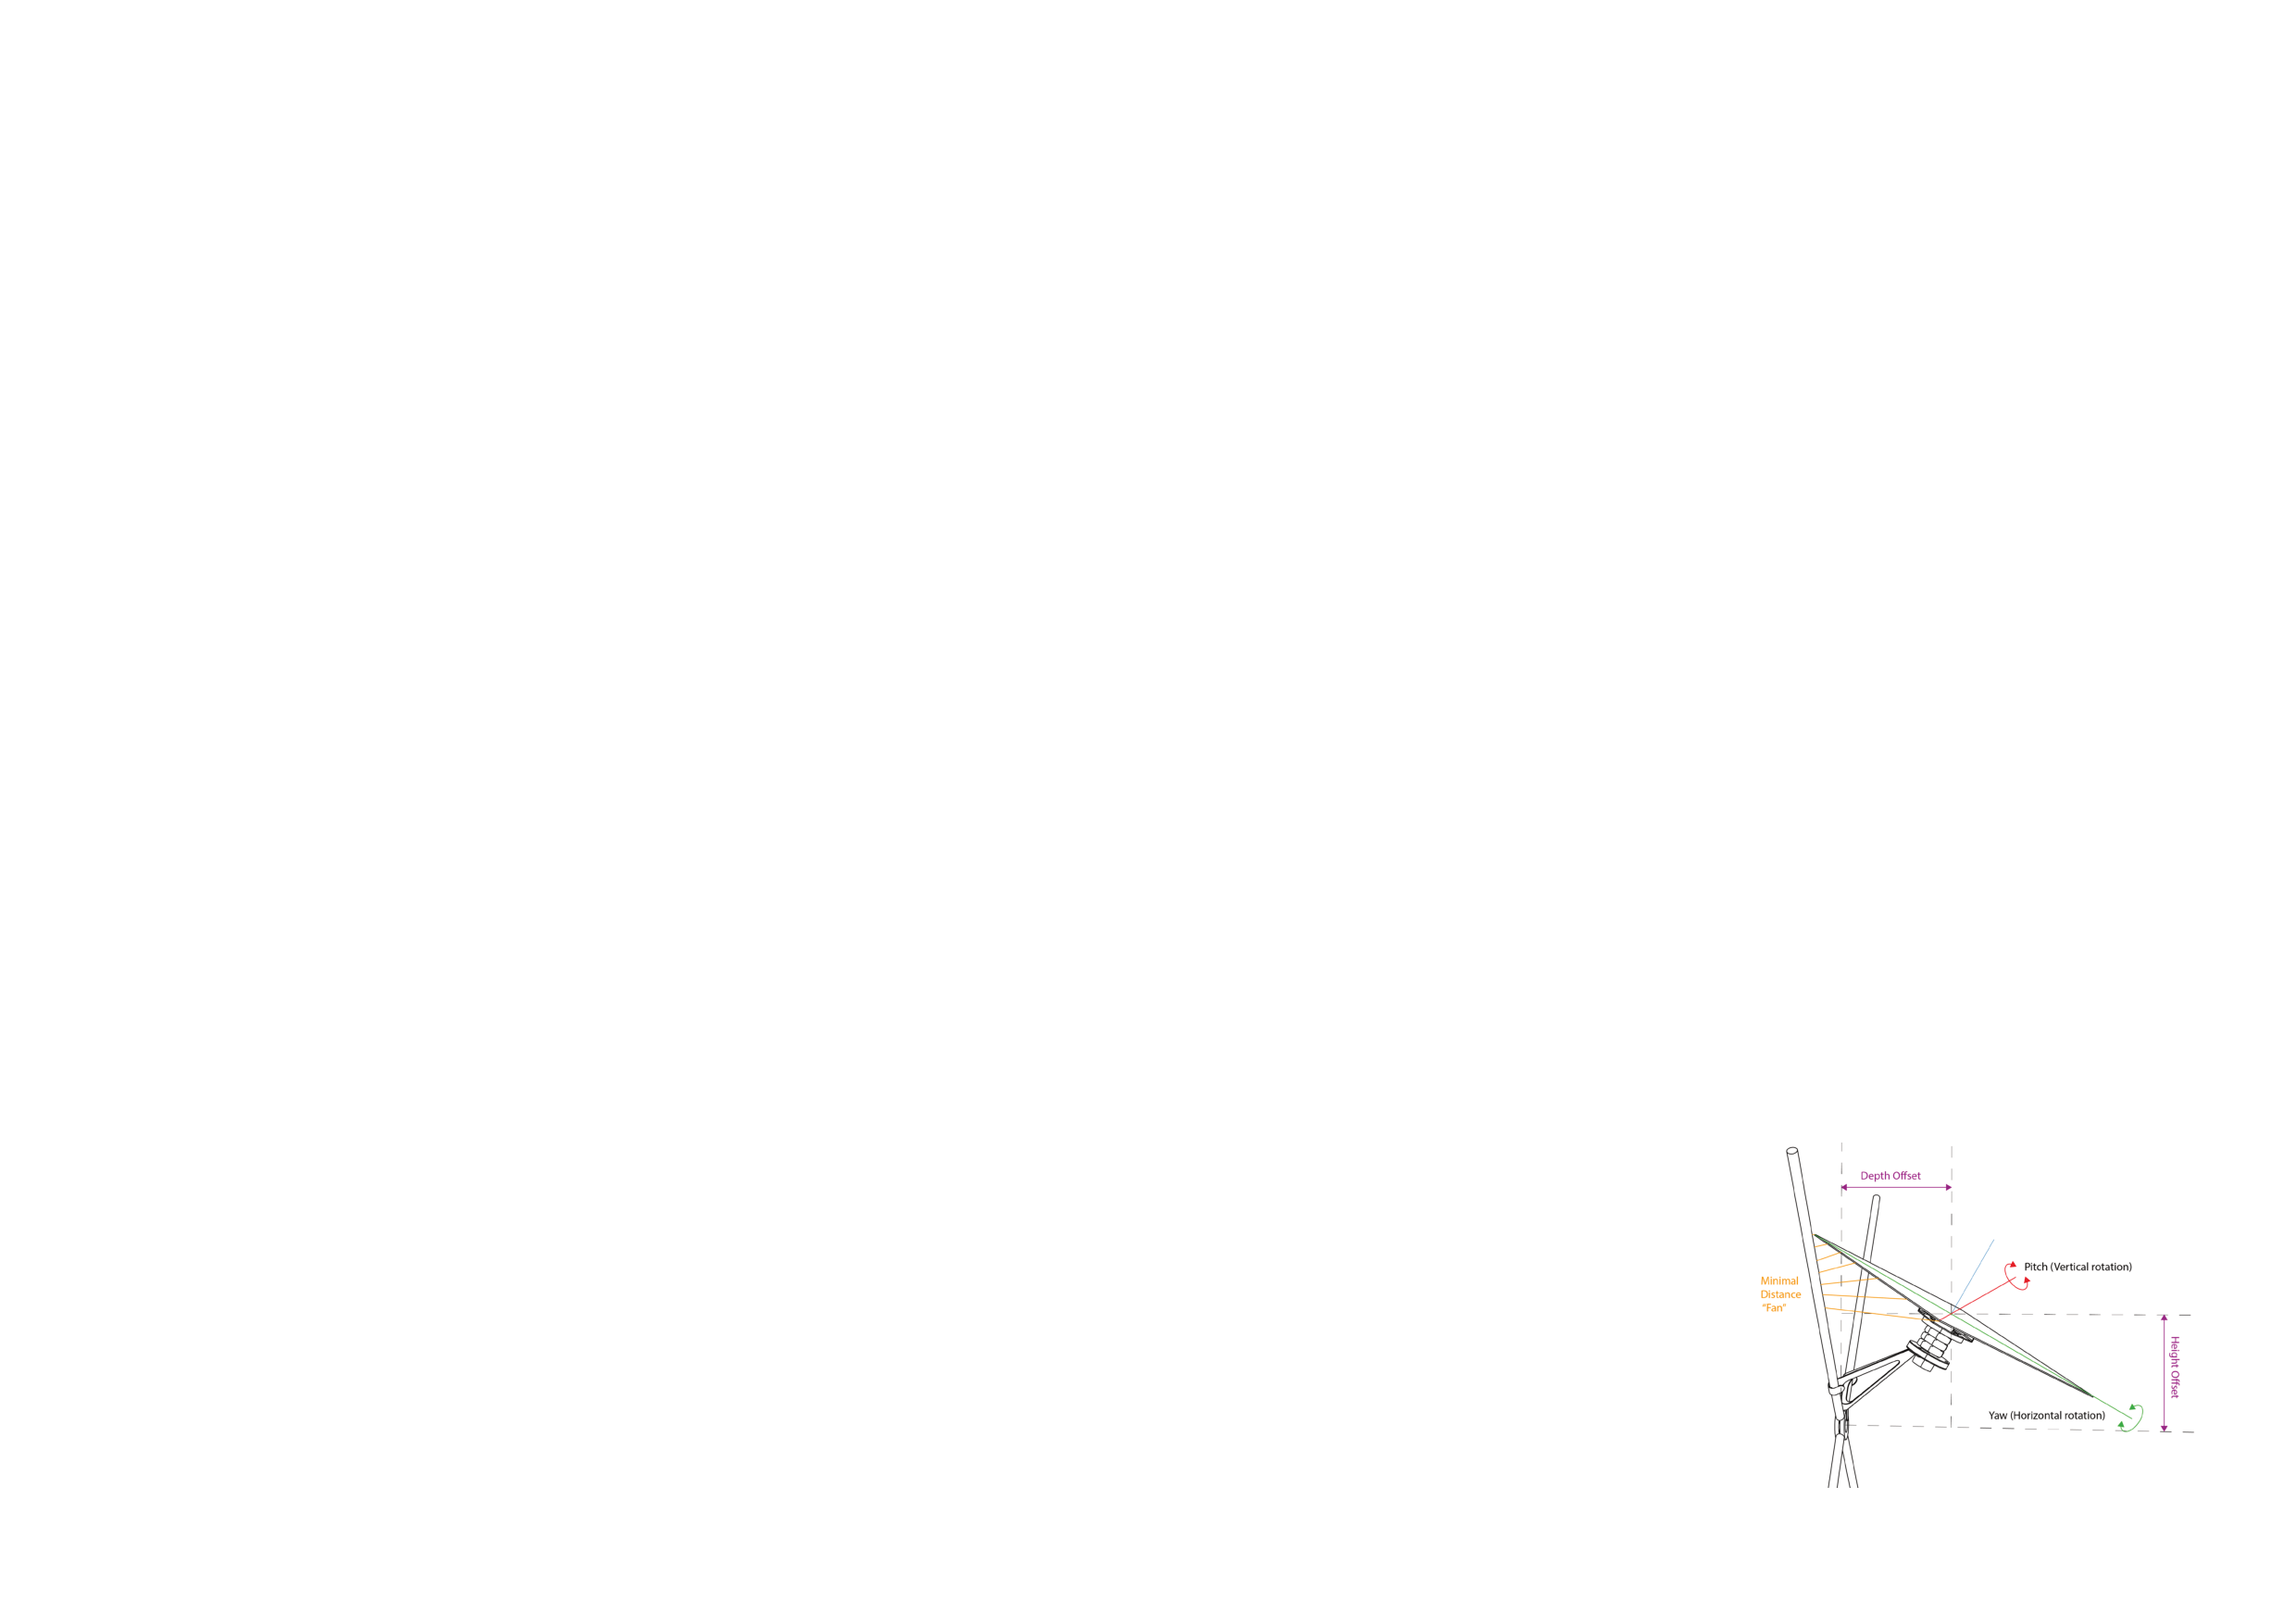
\includegraphics[width=\columnwidth, trim= 0cm 0cm 0cm 0cm,clip]{panelconstraints.pdf}
\caption{Constraints of panel motion relative to the structure}
\label{fig:constraints}
\end{center}
\end{figure}

\begin{figure}
\begin{center}
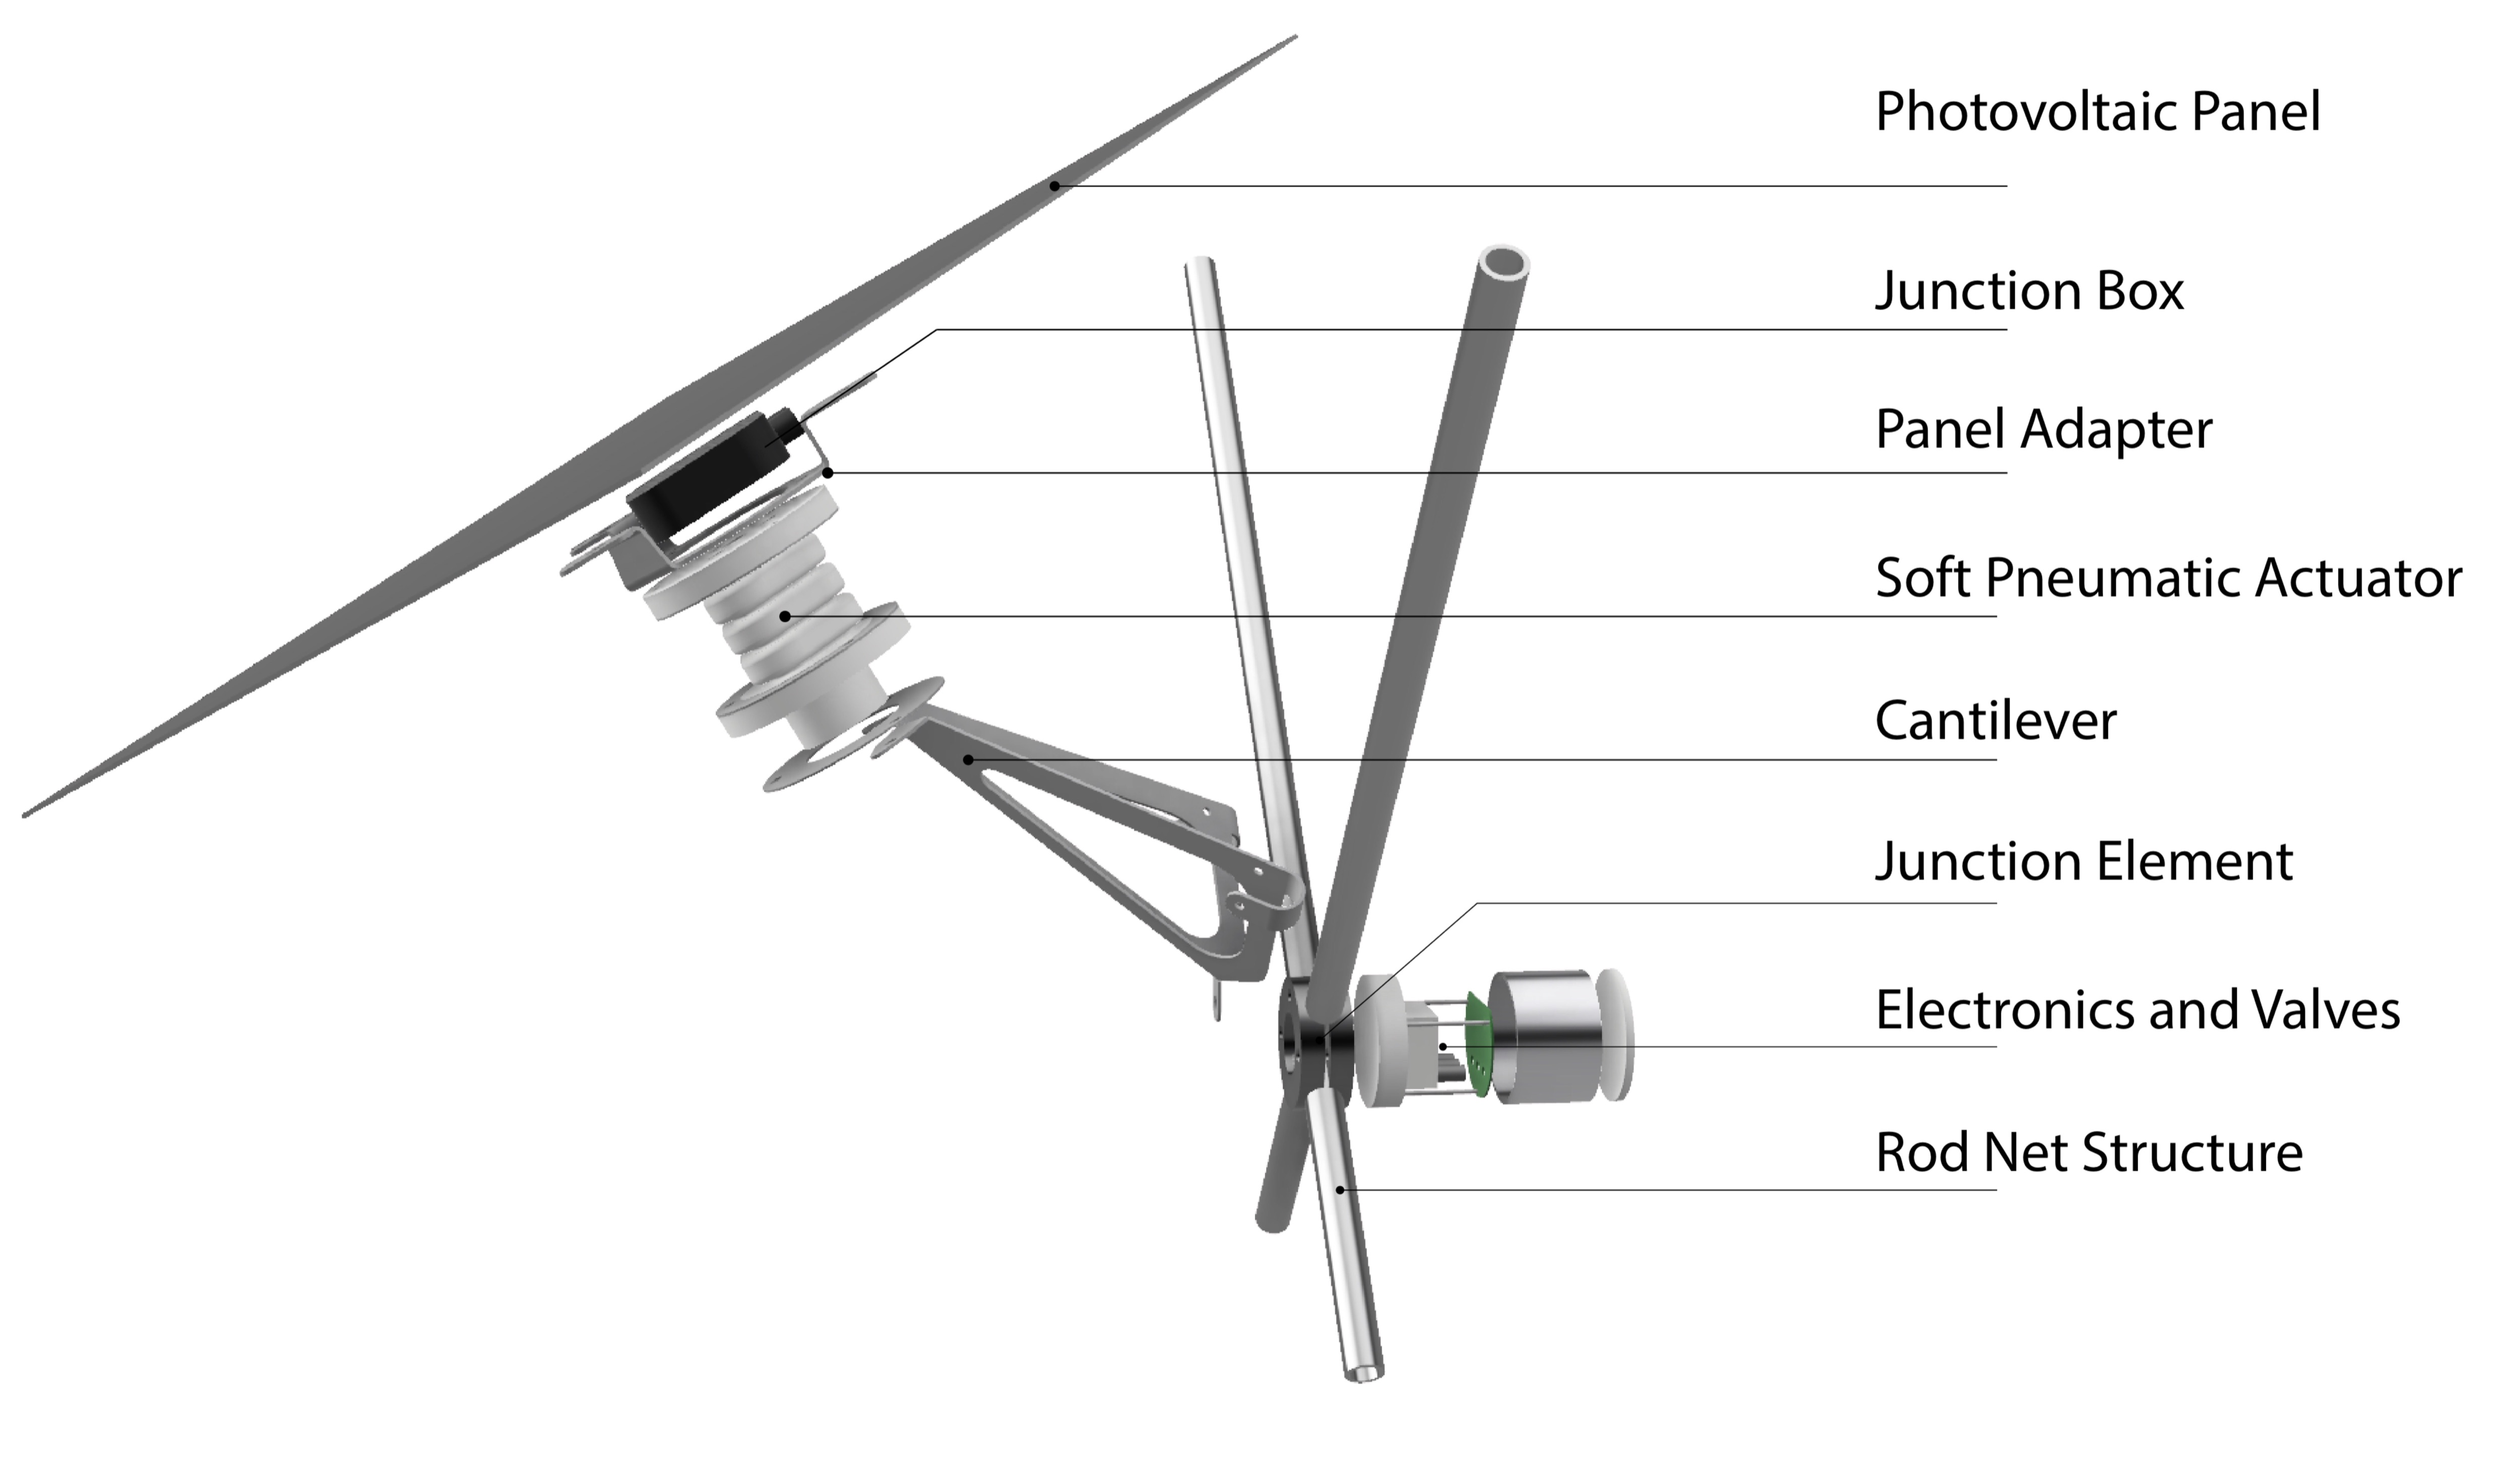
\includegraphics[width=\columnwidth, trim= 0cm 0cm 0cm 0cm,clip]{ExplodedView2.pdf}
\caption{Exploded View of the final ASF Module}
\label{fig:exploded}
\end{center}
\end{figure}

\subsection{Fabrication}

Once a design has been configured using the PDE, manufacturing plans can be automatically generated. This enables the plans to be immediately sent to manufacturers, without a significant time investment. This is especially important for components such as the steel pipes where each pipe has a unique length and bend angle. As an example, Figure \ref{fig:pipeplans} details four of the 92 pipe bending plans. Besides the plan, the PDE also generates a set of meta data that can be directly fed into a CNC pipe bending machine, thus simplifying the transition from design to production.  

An ASF for the HiLo building was fabricated for testing purposes. The overall system took two people 11 days to construct, and was mounted onto a temporary concrete wall in one day, as seen in Figure \ref{fig:mounting}. The design generated by the performative design environment was flawless. The ASF is currently undergoing tests to measure the electricity generation and adaptive control strategy. 

\begin{figure}
\begin{center}
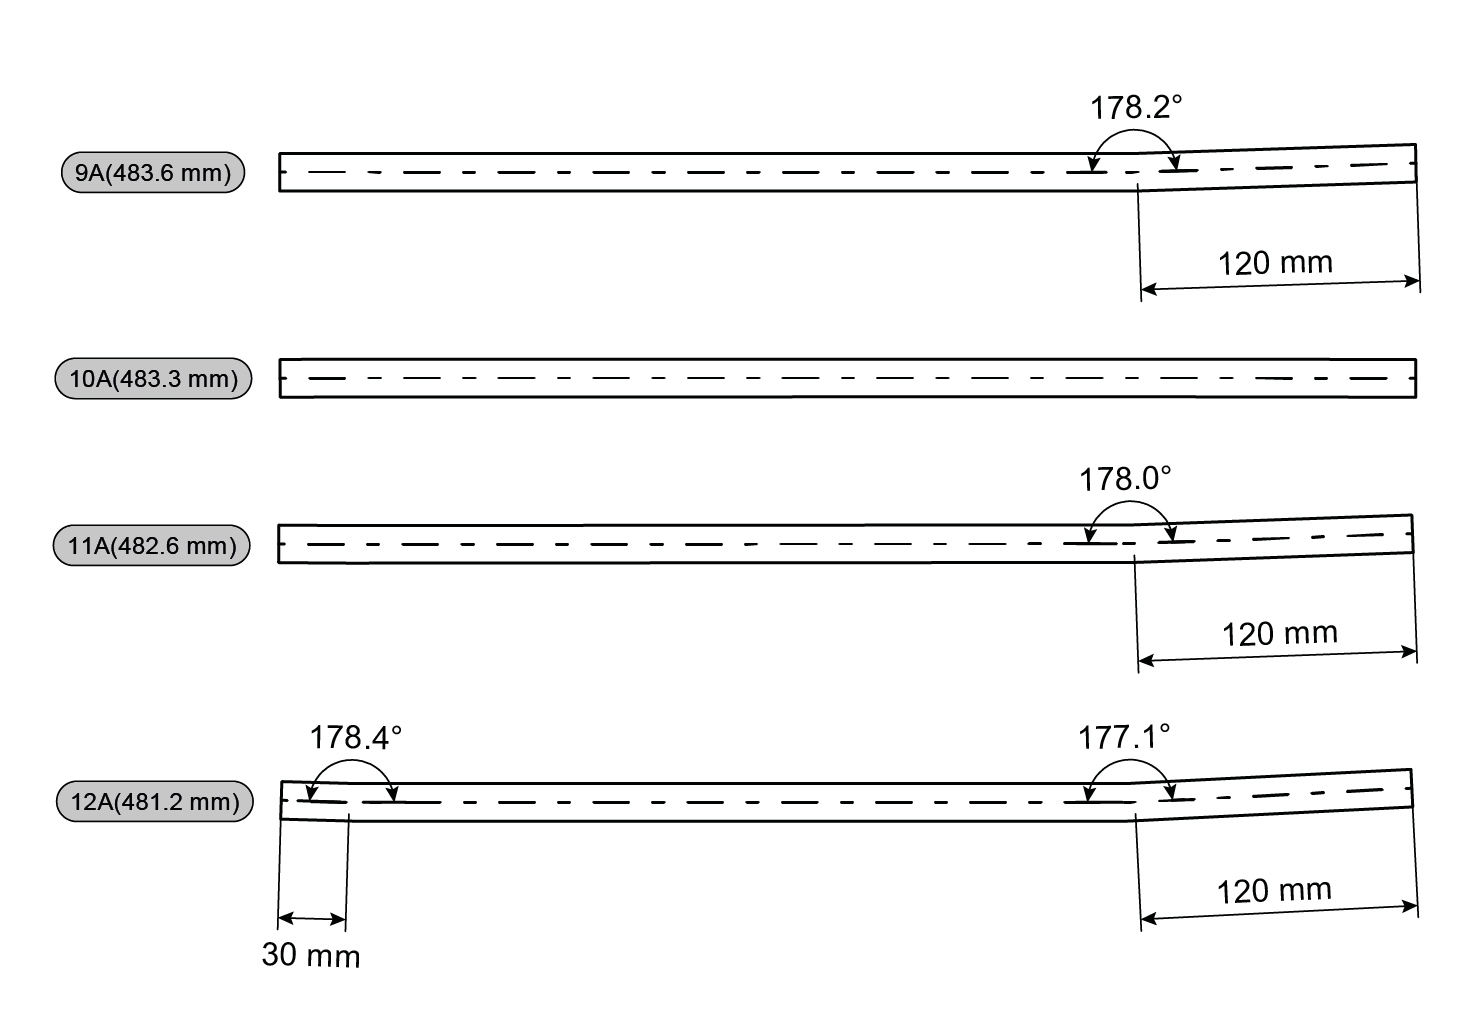
\includegraphics[width=\columnwidth, trim= 0cm 0cm 0cm 0cm,clip]{HiLo_ASF_Pipe_Plans.png}
\caption{Automatically generated drawings for pipe bending. Here we show four of the 92 pipe drawings}
\label{fig:pipeplans}
\end{center}
\end{figure}

\begin{figure}
    \centering
    \begin{subfigure}[b]{0.47\textwidth}
        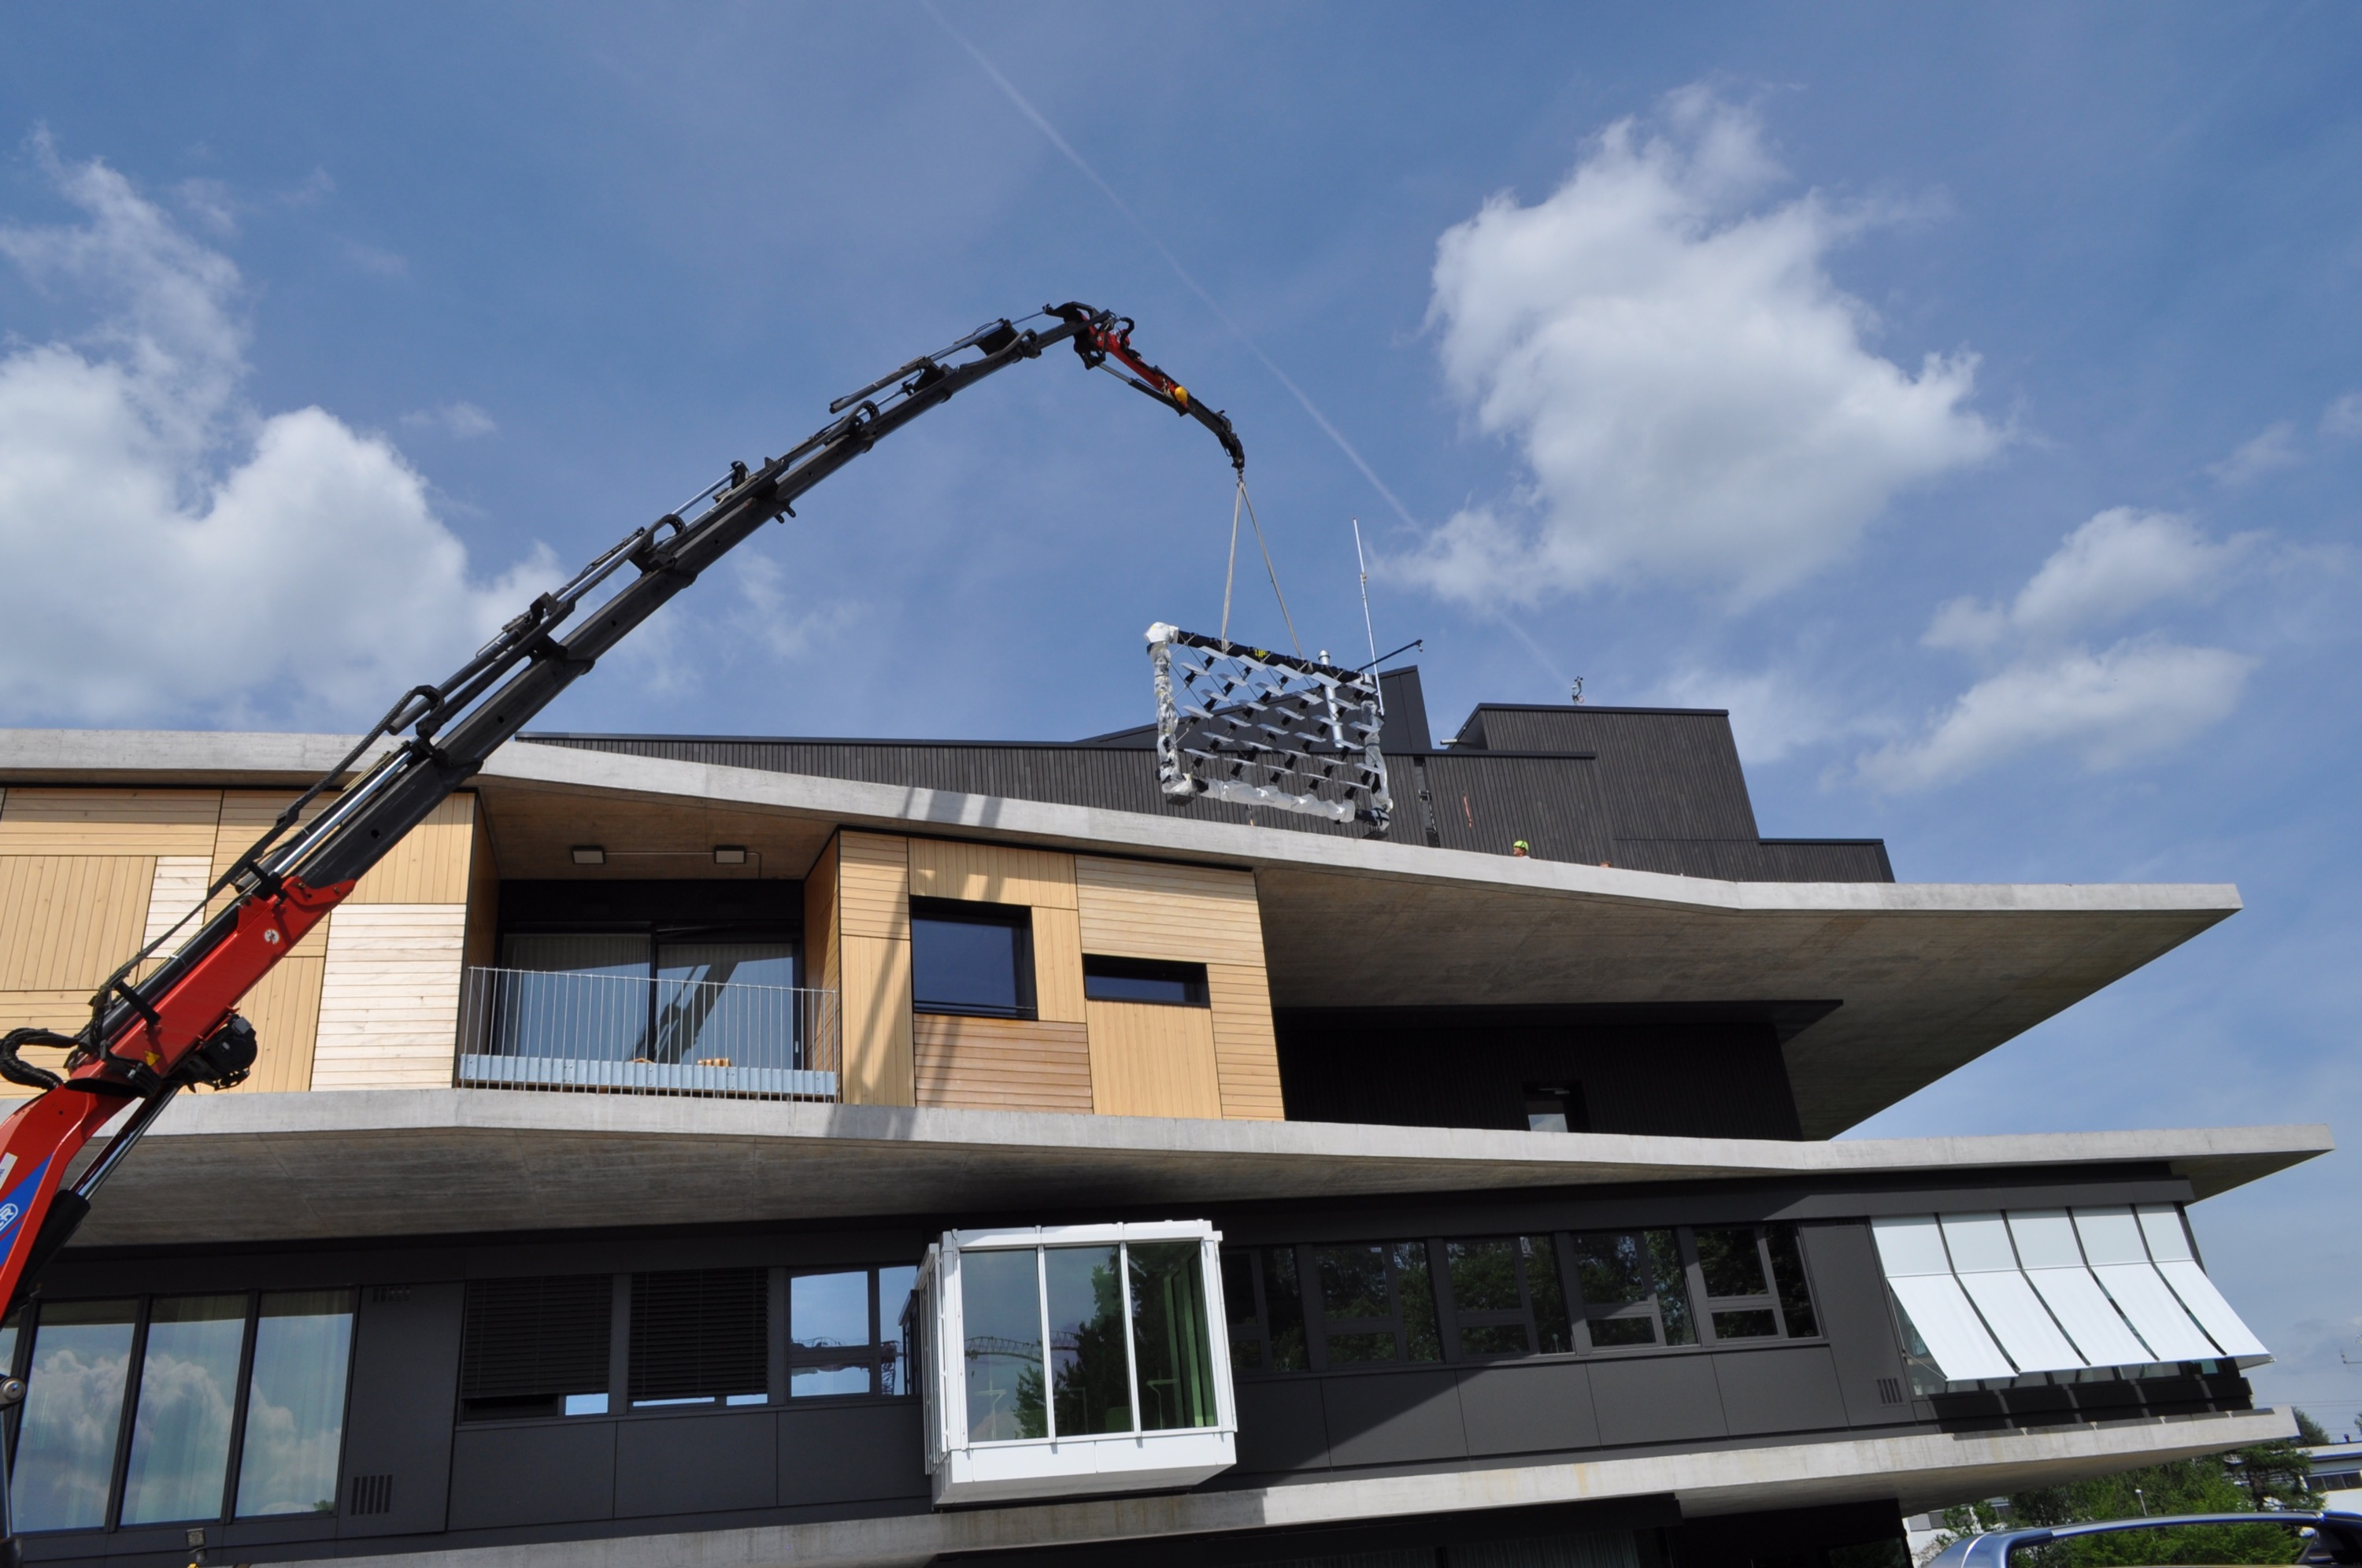
\includegraphics[width=\textwidth]{mounting.JPG}
        \caption{} 
        \label{fig:mountingCrane}
    \end{subfigure} 
    \begin{subfigure}[b]{0.47\textwidth}
        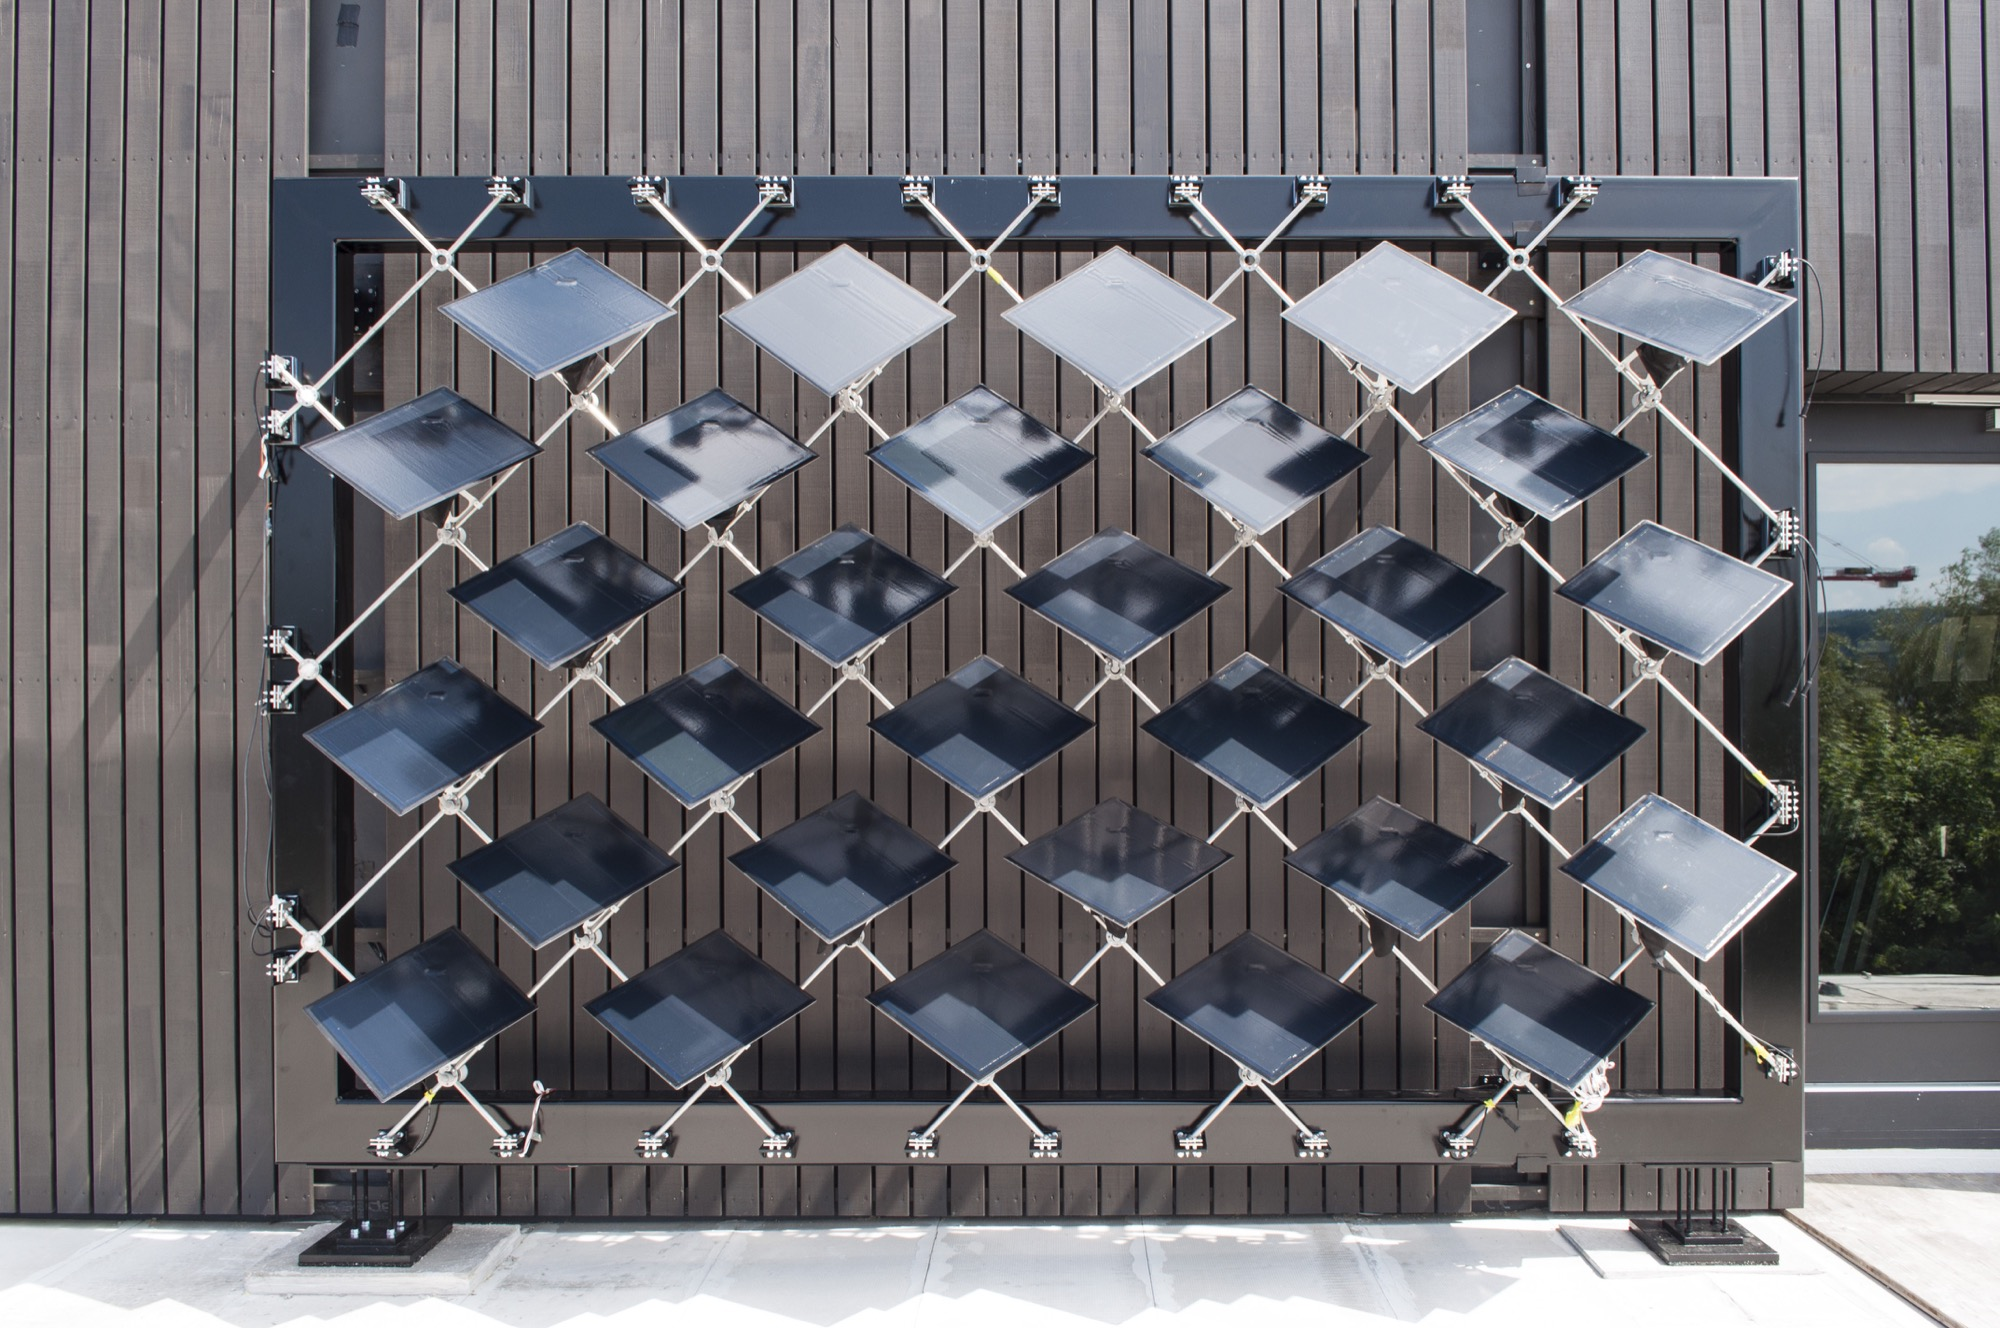
\includegraphics[width=\textwidth]{ASFFront.jpg}
        \caption{}
        \label{fig:mountingFront}
    \end{subfigure}
    \hfill

    \caption{Mounting of a prefabricated ASF to the test site.}
    \label{fig:mounting}
\end{figure}